% !TeX spellcheck = en_US 
\chapter{Methodology}\label{MET}
This chapter discusses the methodology that uses load sequences that ended in fatigue failure, to get a confidence value for the accumulated damage sum D of a load sequence that did not yet end in failure. Each step of the proposed method is discussed in detail. Chapters \ref{DA} and \ref{DV} give an introduction to the data, while chapter \ref{GO} serves as general guidance. Detailed explanations begin in chapter \ref{SBOC}.

\section{Data Acquisition}\label{DA}
The load sequences are acquired by performing a Single Tooth Bending Fatigue Test (STBF). A gear is held in place by two teeth clamped in a test rig. A hydraulic piston is applying cyclical loading until bending fatigue failure occurs. The loading profile is manually defined for each test. The loading profile consists of a force level and the number of cycles during which this force is applied. Instead of constructing the loading sequence from the predetermined parameters (force and repetitions), a force sensor is used that records the net force of a cycle that occurs at its peak. This is done to simulate real machinery, where the loading history is also measured and not created by a-priori available hyperparameters. 
Figure \ref{fig:STBFT} shows an exemplary test rig for STBF tests.
\begin{figure}[H]
	\centering
	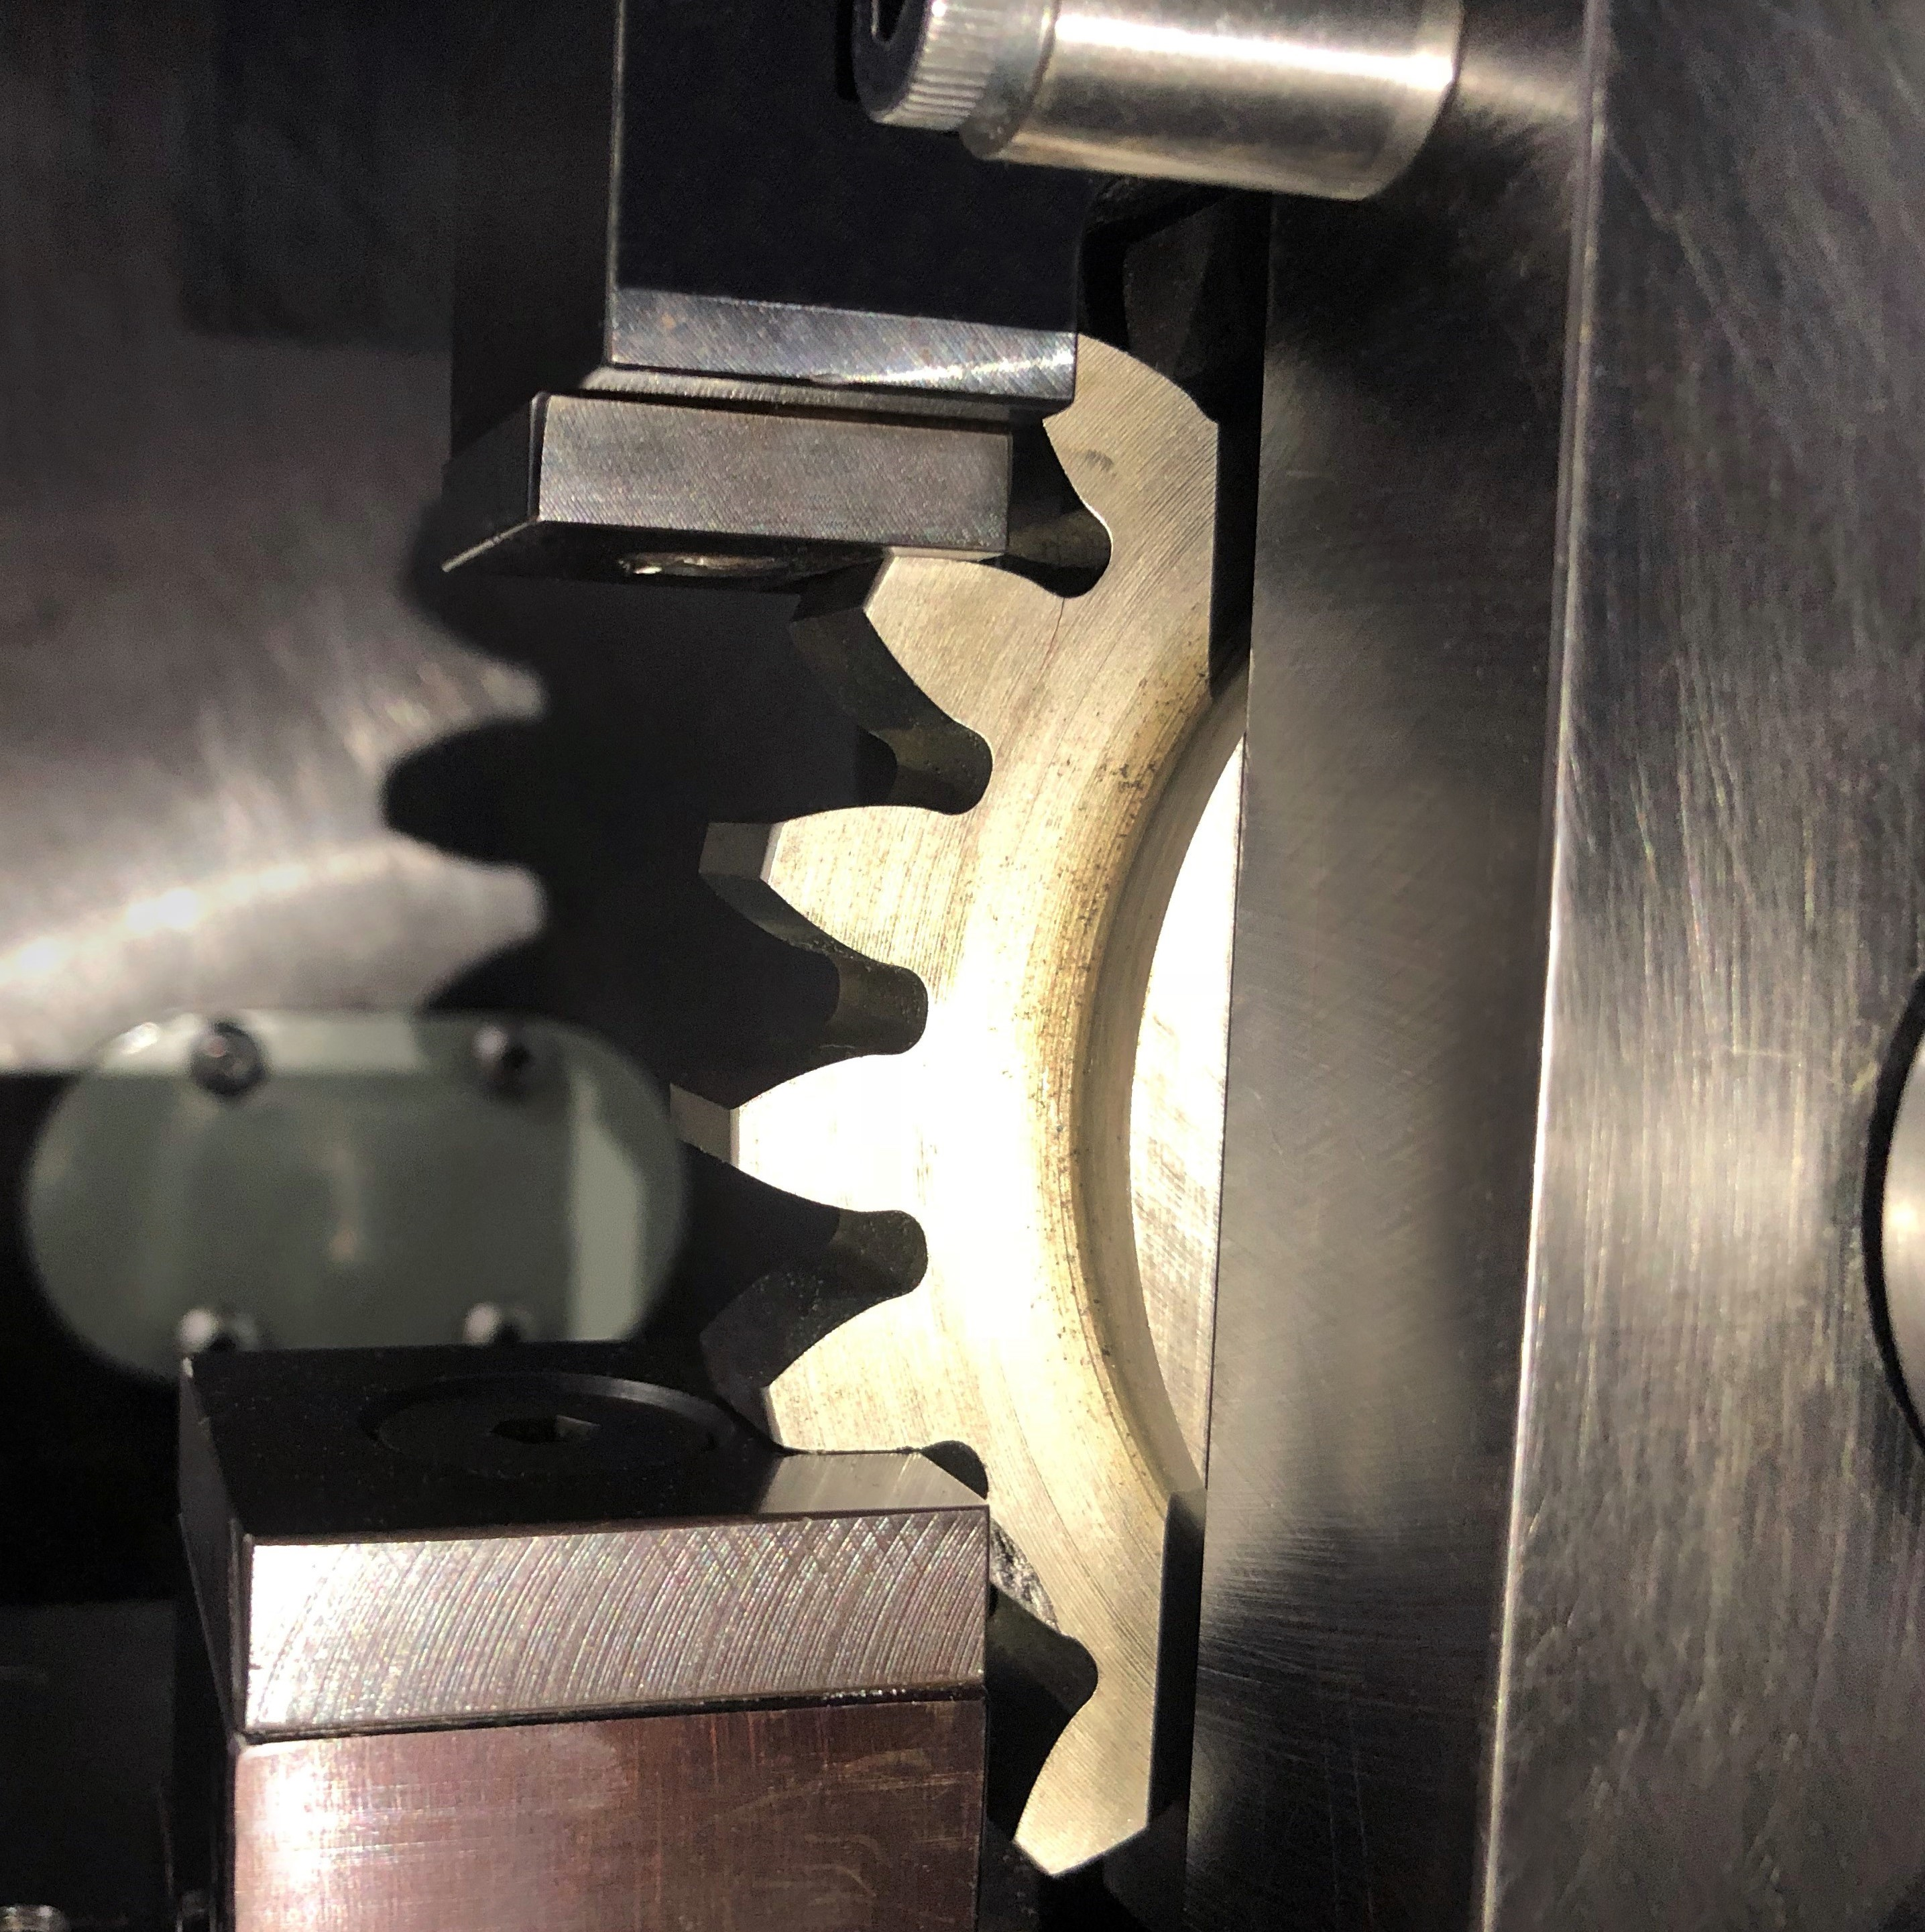
\includegraphics[width=0.5\linewidth]{IMGs/tooth.jpg}
	\caption{Test rig for Single Tooth Bending Fatigue Test \cite{STBT}}
	\label{fig:STBFT}
\end{figure}
\newpage
\section{Data Visualization}\label{DV}
Figures \ref{fig:L1}, \ref{fig:L2} and \ref{fig:L3} show three different load sequences. The \(x\)-axis denotes the number of the cycle in that sequence, and the \(y\)-axis the applied force. As the force is acting in the negative direction with regard to the defined coordinate system, it is recorded with a negative sign. The clamping force is set to 3 kN. The sudden reduction of force in the load history appears when the test rig switches from one load-level to another. 
Additionally, the vertical lines represent the damage sum D according to Miner at 0.5, 0.8 and 1. Note that failure is expected at a damage sum equal to 1. The tested gear with the load sequence presented in figure \ref{fig:L2} was able to accumulate a damage sum D greater than unity, and is thus exceeding its expected failure point. The applied load sequence shown \ref{fig:L3} resulted in early failure.

\begin{figure}[H]
	\centering
	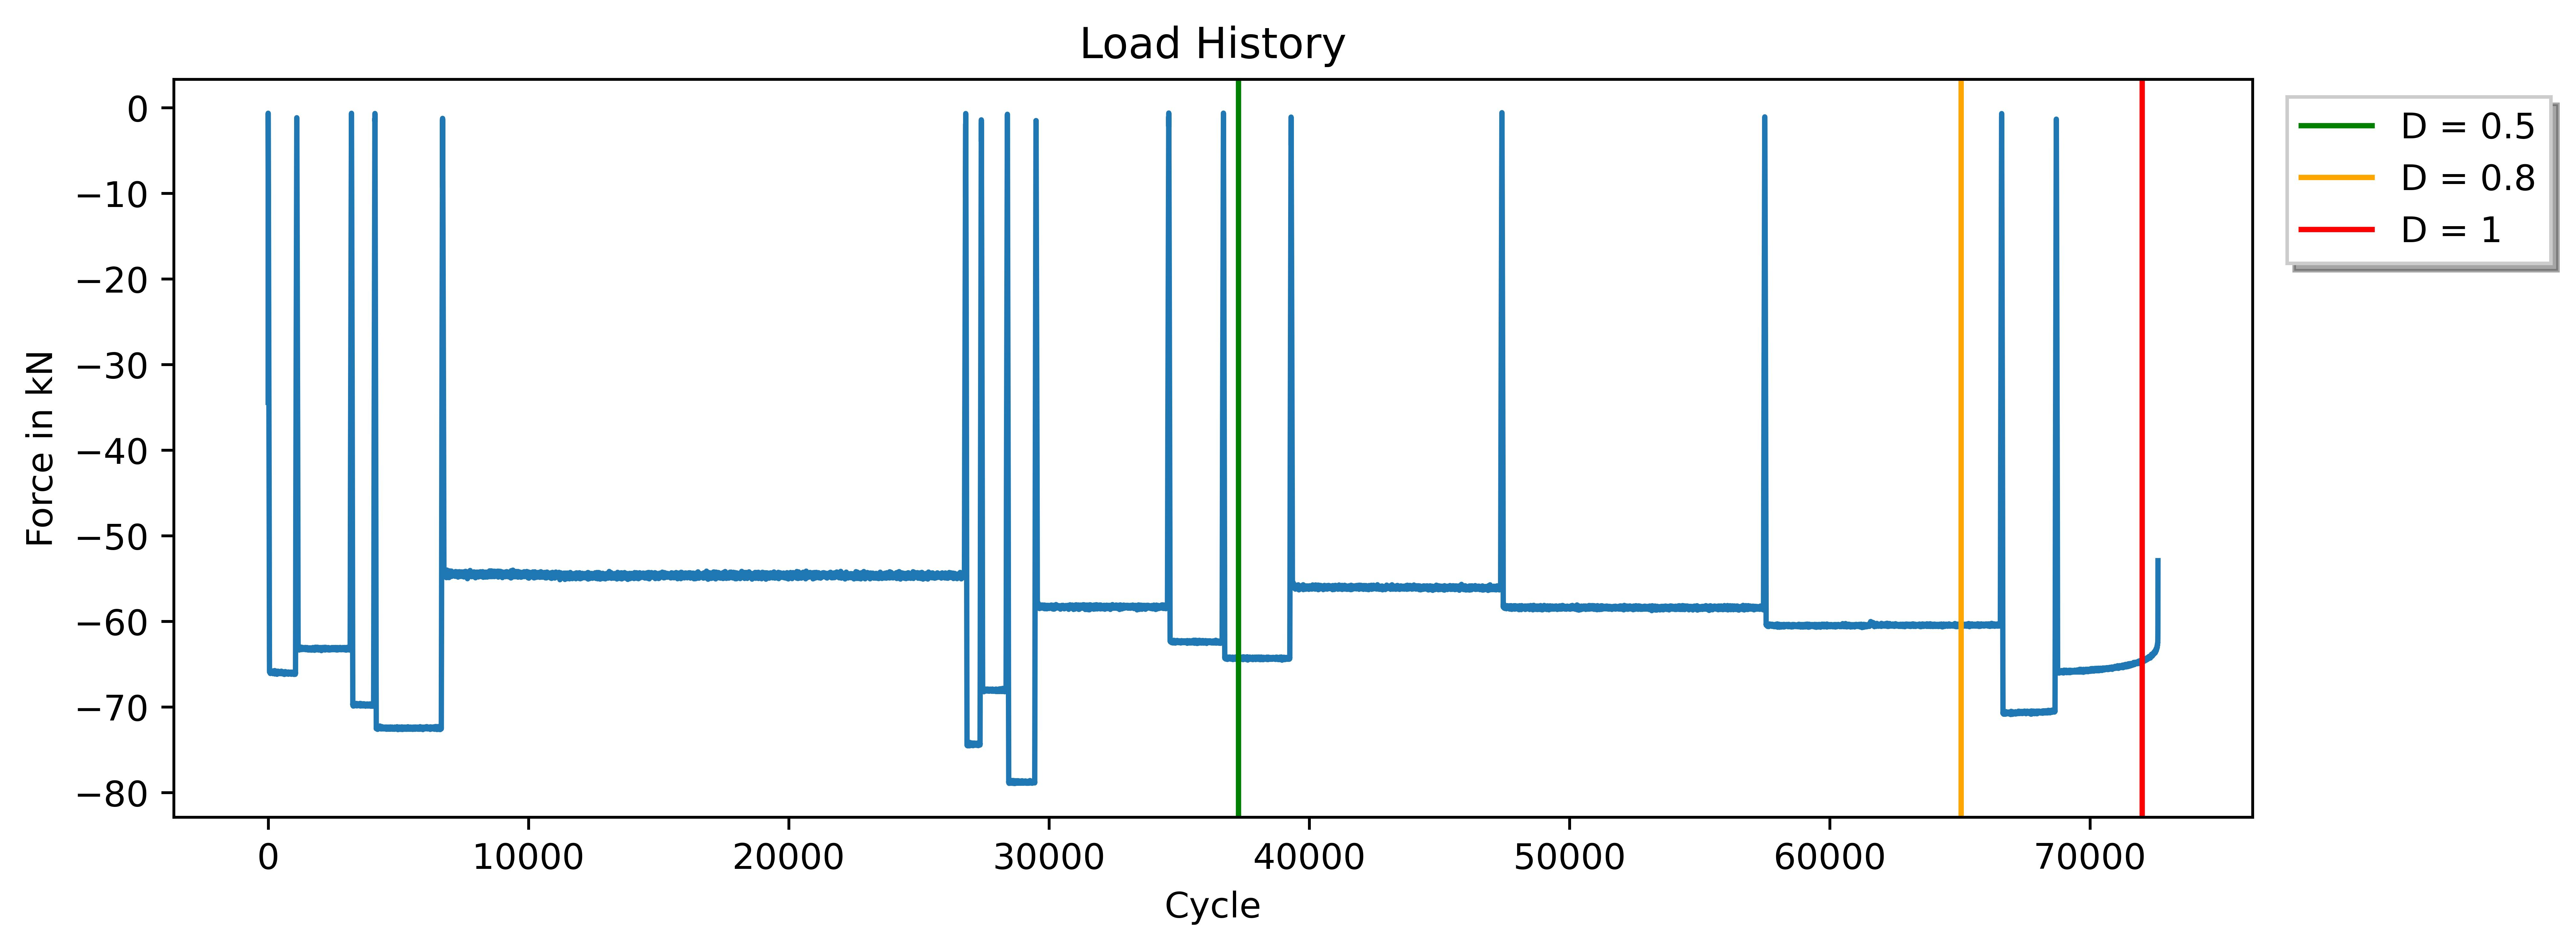
\includegraphics[width=1\linewidth]{IMGs/Load/L0.jpg}
	\caption{Load sequence with failure close to D=1}
	\label{fig:L1}
\end{figure}

\begin{figure}[H]
	\centering
	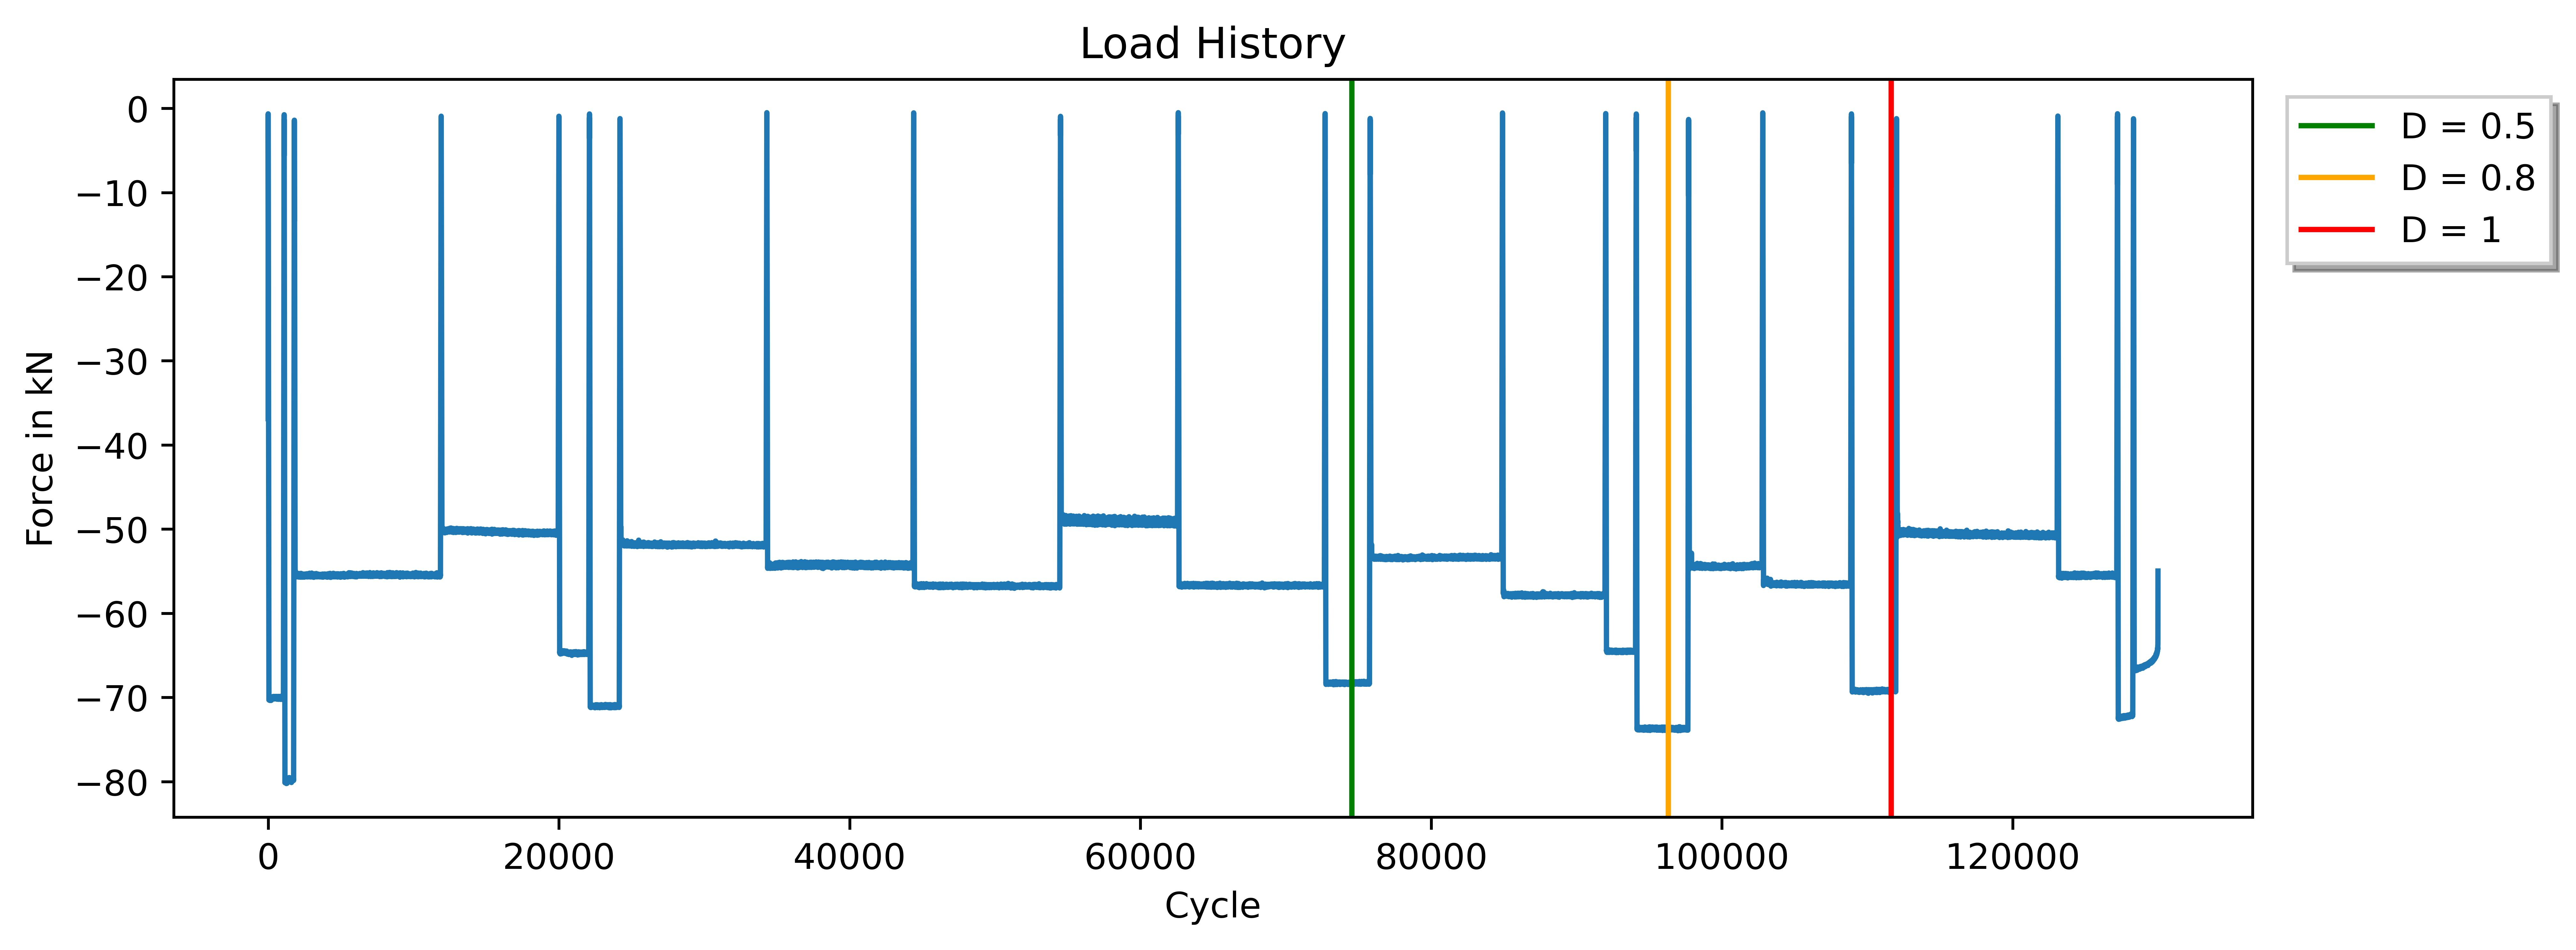
\includegraphics[width=1\linewidth]{IMGs/Load/L1.jpg}
	\caption{Load sequence with failure at D>>1}
	\label{fig:L2}
\end{figure}

\begin{figure}[H]
	\centering
	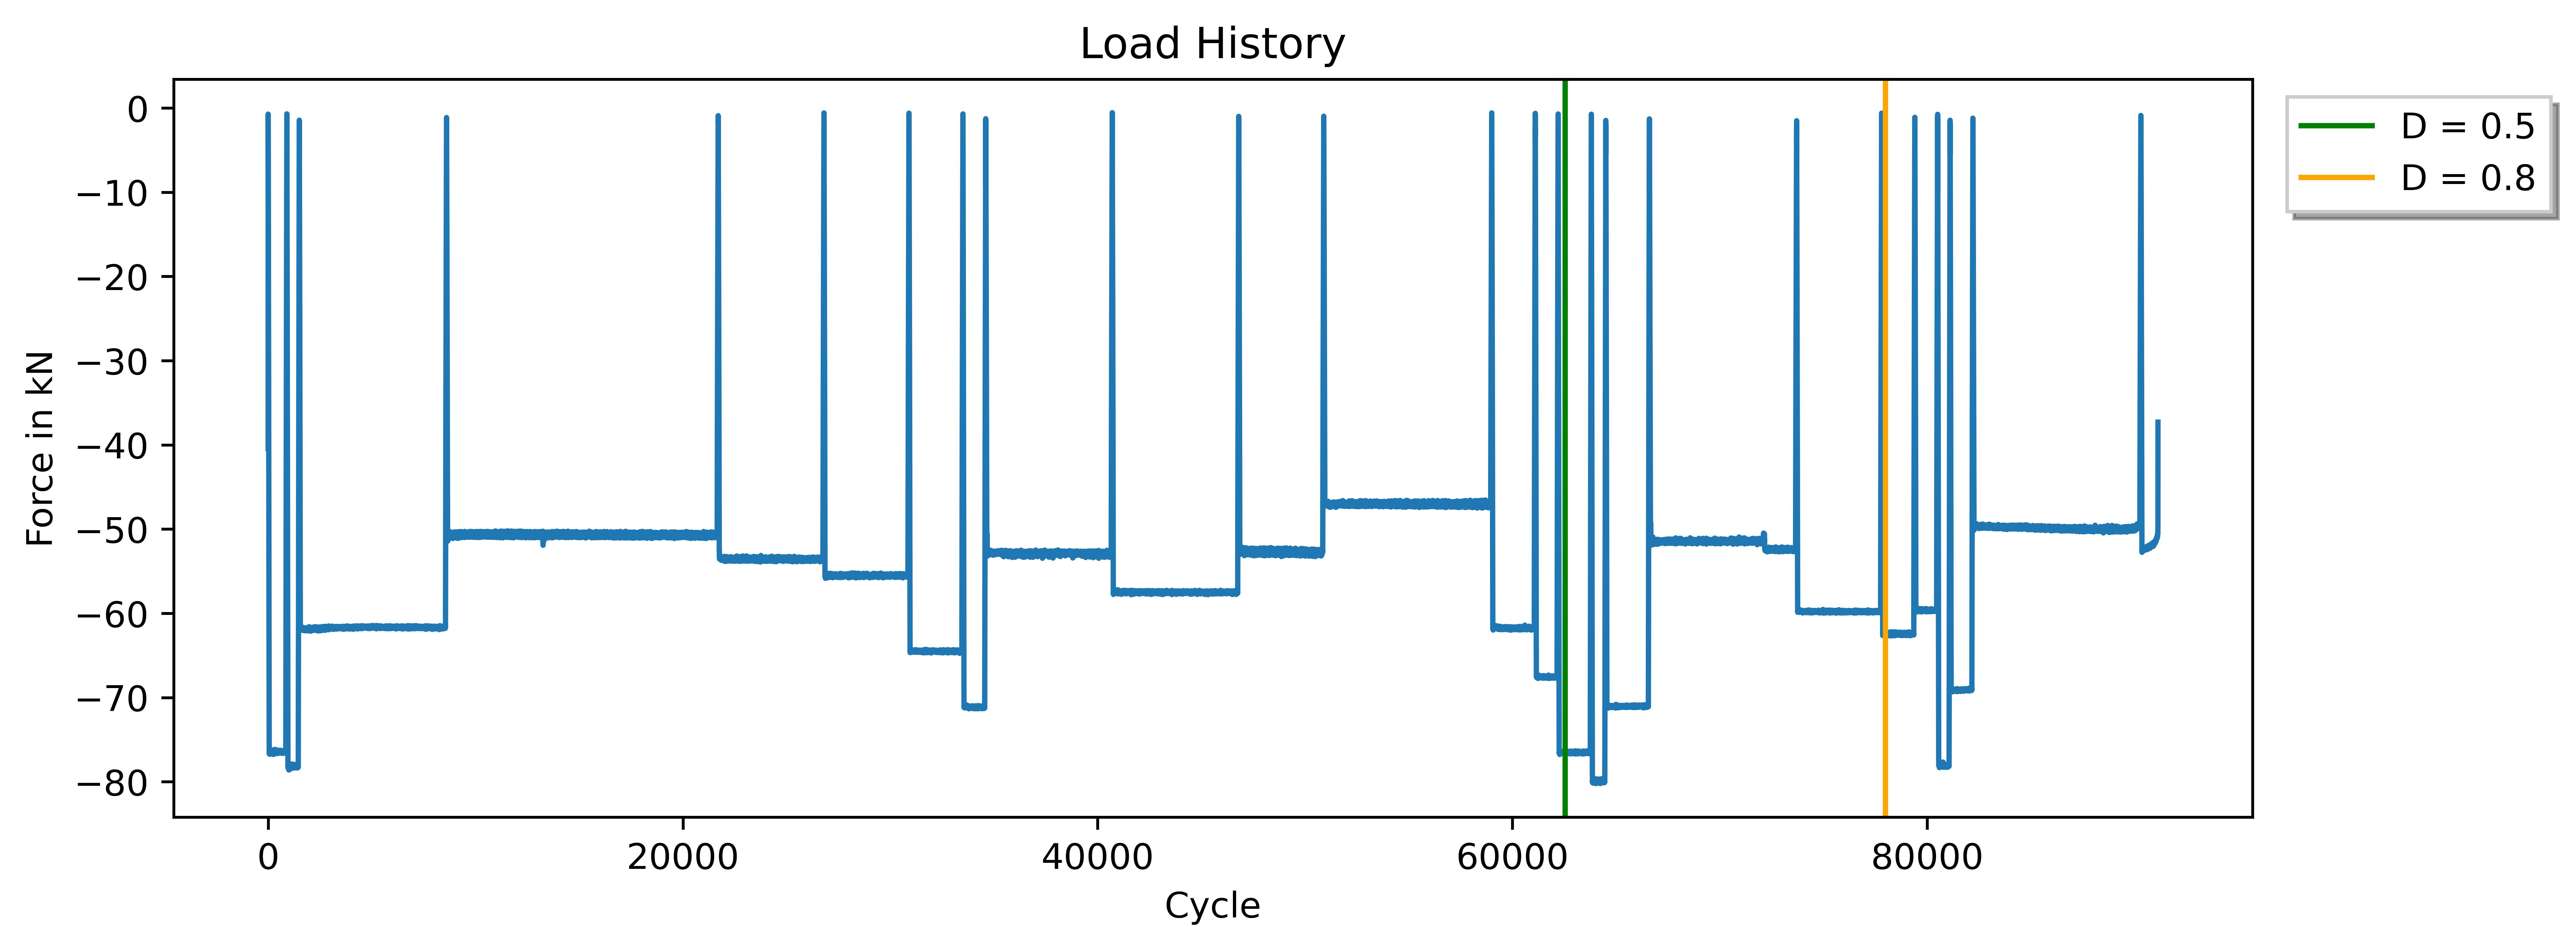
\includegraphics[width=1\linewidth]{IMGs/Load/L2.jpg}
	\caption{Load sequence with failure at D<<1}
	\label{fig:L3}
\end{figure}

Note that for a ML approach, the absolute values are irrelevant and can be changed as long as all load sequences are transformed in the same way. Flipping the sign or dividing by a constant to get the stress per unit area will result in equal performance of the selected method.

\section{General Overview of the Proposed Structure}\label{GO}
The first goal is to use a classifier to determine if a load sequence will result in early (D<1), late~(D>1) or on-time failure (D$\approx$1). In other words, if a load sequence is more or less damaging than assumed by the Miner-Rule, based on the order of the loads. Based on that knowledge, it is possible to deduce the confidence in the damage sum D that was calculated with the Miner rule. For example, if the load sequence is classified as part of the less damaging ones, it is fair to assume that the Miner rule gives a conservative estimate of the actual physical damage. 

After that, a regression is performed to estimate a new defined health indicator called "State of Health" (SOH). 
Figure \ref{fig:GeneralMethod1} shows the process of classifying a load sequence with unknown effects based on the available load sequences that are used as training data. 

\begin{figure}[H]
	\centering
	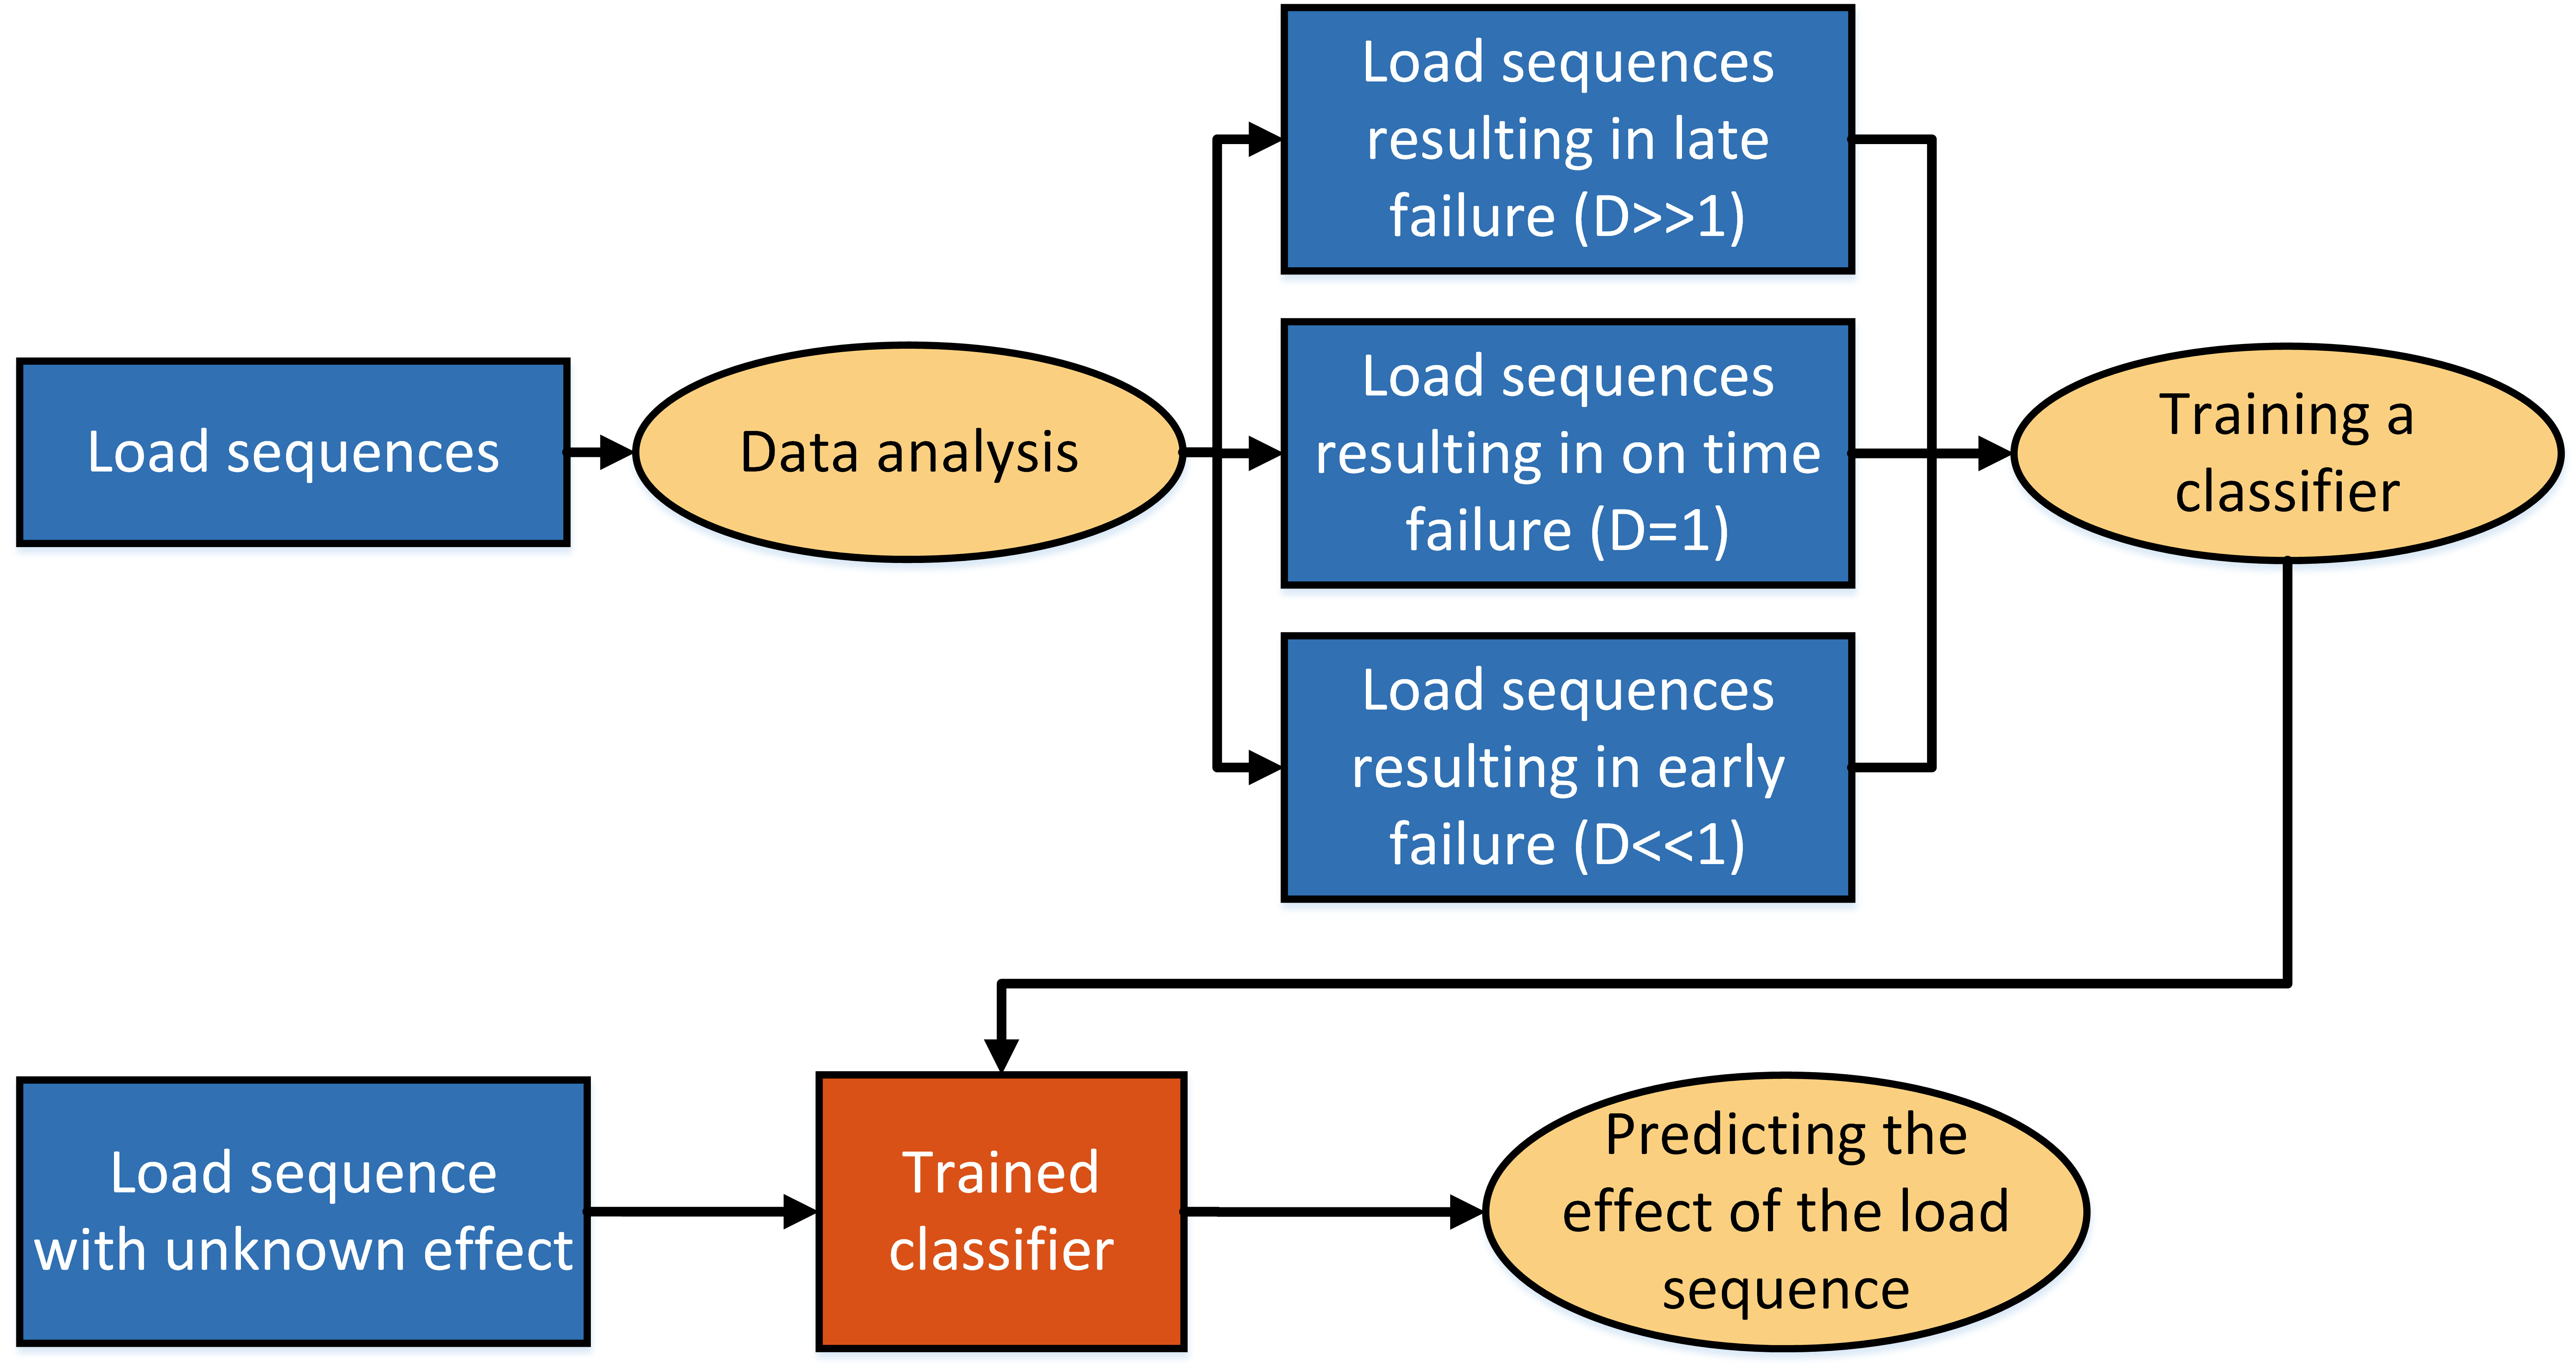
\includegraphics[width=0.95\linewidth]{IMGs/Method1.png}
	\caption{Methodology for classifying a load sequence with unknown effect}
	\label{fig:GeneralMethod1}
\end{figure}

The SOH is not to be confused with a RUL prediction. SOH is comparable to a cars' notification that, for example, the brakes are 80\% worn down and will soon require a maintenance visit to the mechanic. 

The SOH prediction is based on similarly damaging load sequences, with a linear interpolation between the starting point of the sequence at 0, and failure at 1. The damage sum is not taken into account in this step. 
Figure \ref{fig:GeneralMethod2} shows a schematic diagram of how a SOH prediction is acquired.
First, a subset of the original datasets is taken where all load sequences have the same damaging effect. %That means that they are either more damaging and thus resulting in early failures, or less damaging, allowing them to run past an accumulated damage sum greater than unity.

The end points of those known sequences are mapped to a linear function starting at 0 at the beginning of the sequence and ending at 1 at the end. This function is referred to as the label-function. Now, the load sequences are cut at different endpoints. The label of the shortened sequences is calculated with the label-function. The label of those snippets is the value of the label-function at the end of a sequence. The shortened sequences and their corresponding labels are combined into a data-set. That data-set is used to train a regressor to predict the SOH of a new sequence. The detailed explanation of the involved steps for predicting the SOH follows in chapter \ref{PrRe}.

Figure \ref{fig:GeneralMethod2} shows a diagram of the proposed structure for the usage of the regressor. 
 
\begin{figure}[H]
	\centering
	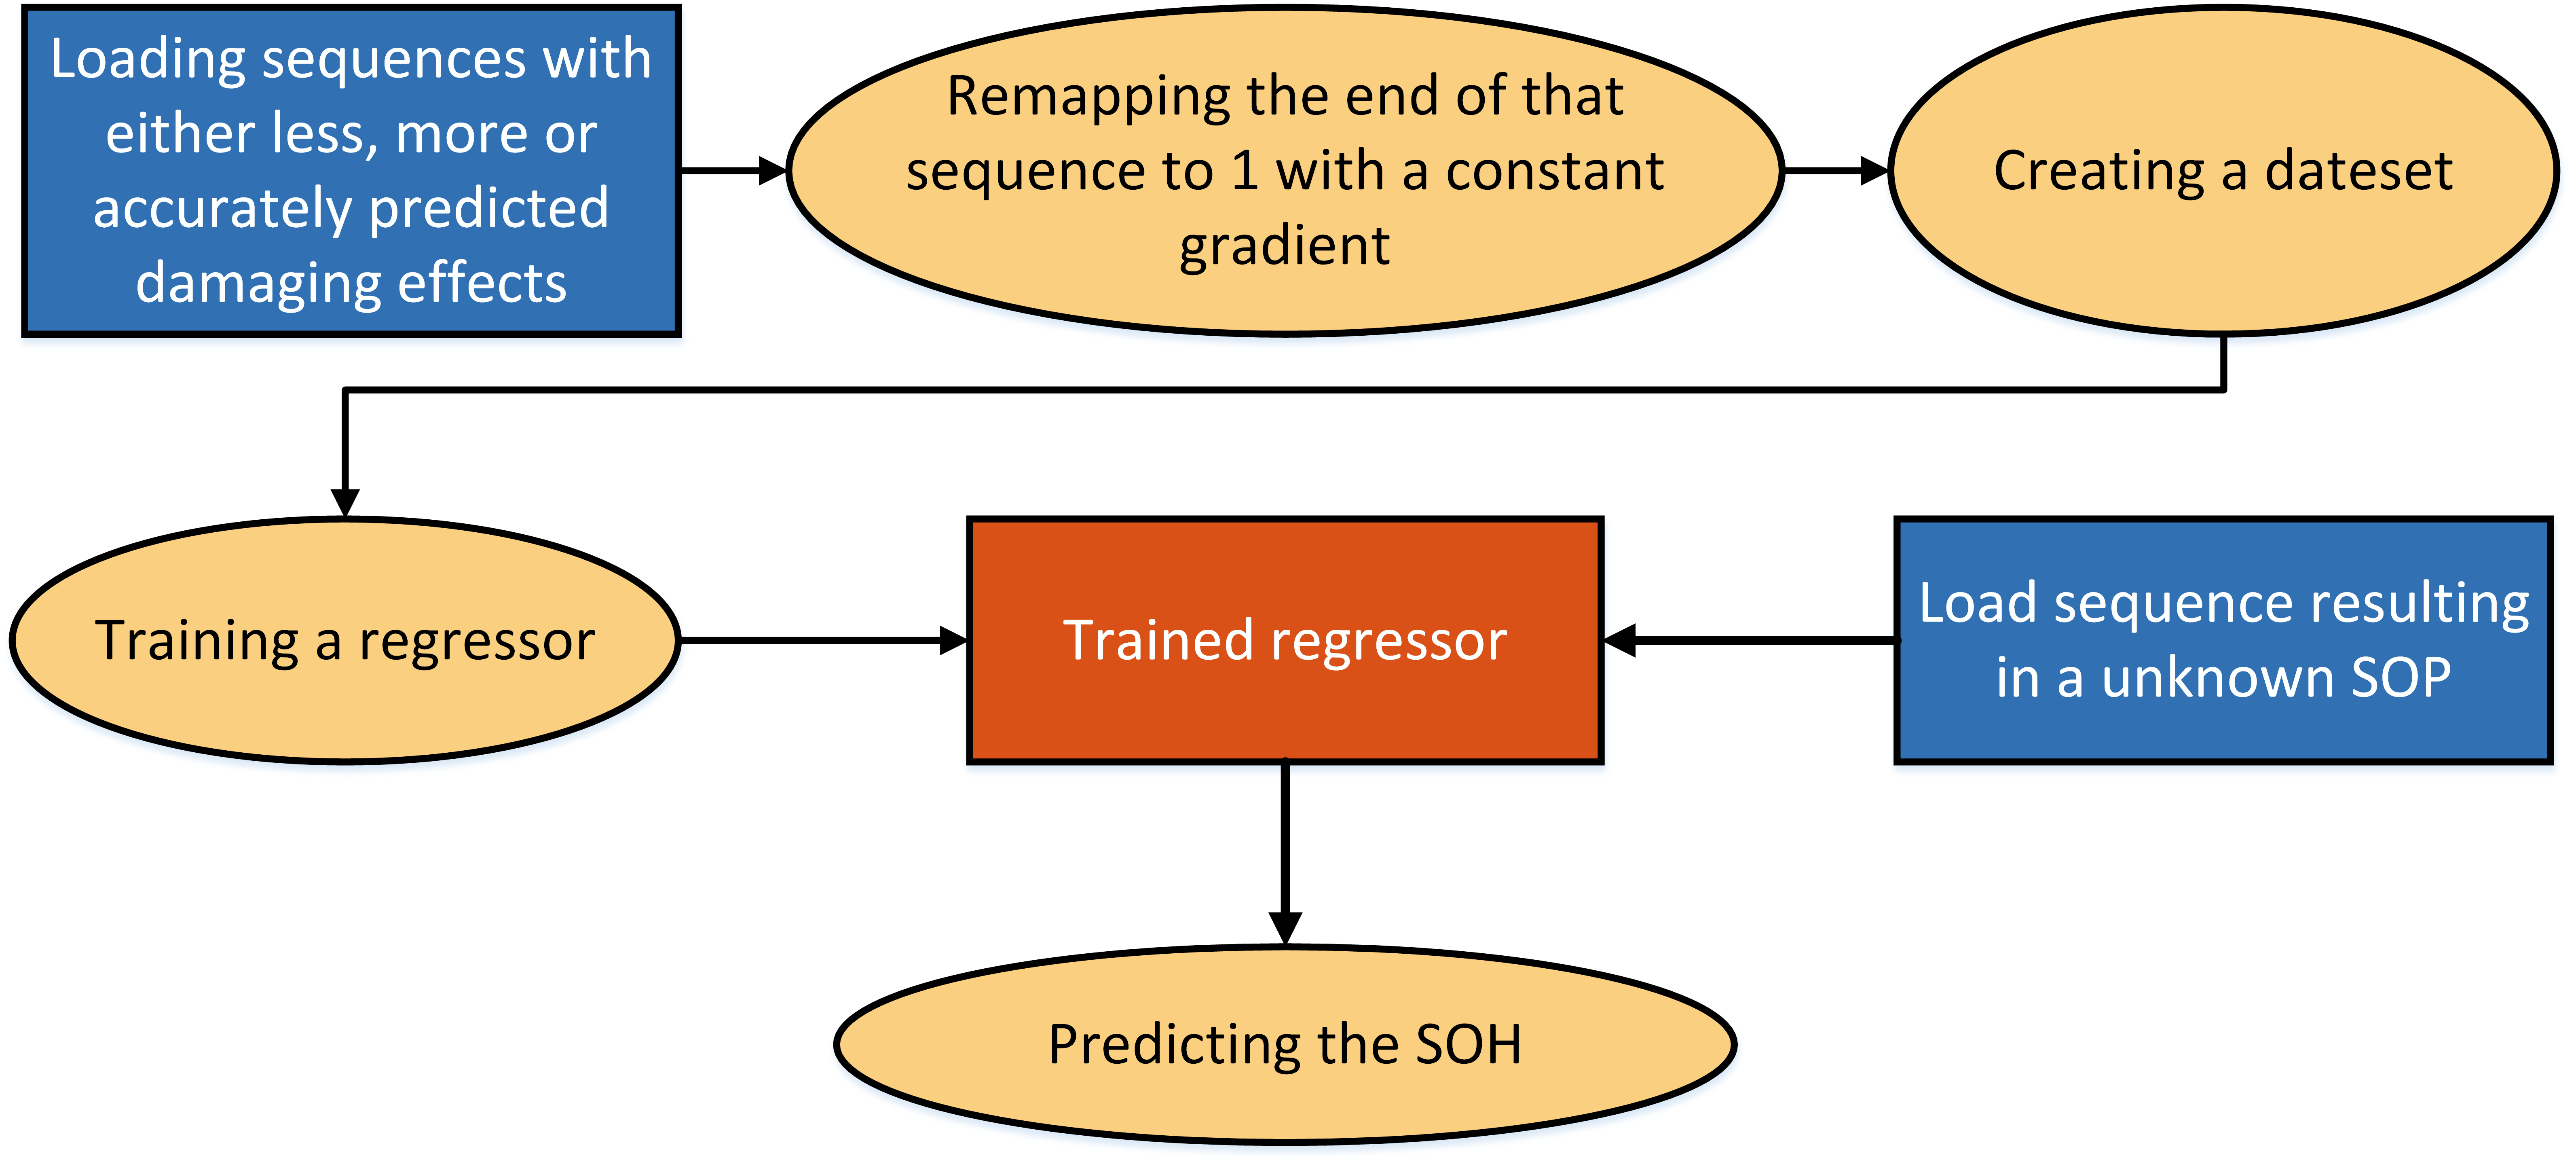
\includegraphics[width=1\linewidth]{IMGs/Method2.png}
	\caption{Methodology for predicting a SOH based on load sequences with similar damaging effects}
	\label{fig:GeneralMethod2}
\end{figure}


In the following, load sequences that have been acquired by STBF are referred to as "finished" load sequences due to the fact that they ended in failure. On the other hand, load sequences that have not yet ended in failure and need to be classified are referred to as "unfinished" load sequences. Only the finished load sequences are used for training the classifier and regressor.


\section{Preparation of the Classifier}
\subsection{Separation based on Class Label}\label{SBOC}
When it comes to classification, it requires a data-set that is labeled (see Chapter \ref{SUPER}). The recordings provided by the experiments do not contain any clear indicators from which the label can be deduced right away. To acquire the label for each individual sequence, the Basquin-Equation \cite{DIN50100} has to be utilized. With the help of this equation, shown in equation \ref{BQ}, the maximum load-cycles (\(N\)), that an element can withstand at a specific load, can be calculated.

The parameters \(C\), \(L_a\) and \(-k\) are constants representing the reference value of fatigue strength, the value of the load at one cycle and the slope of the S-N fatigue strength curve \cite{SOLID}. 
\begin{equation}\label{BQ}
	N = {C}*{L_a}^{-k}
\end{equation}
Inputting the result from equation \ref{BQ} in equation \ref{acc} (from chapter \ref{LAD}) will return the accumulated damage sum D. Figure \ref{fig:SBC} shows the required steps on how the unlabeled load sequences are analyzed and sorted into categories based on the resulting damage sum D. The class labels and the appropriate range of damage sum D are shown in table \ref{DamageClass}.

\begin{figure}[H]
	\centering
	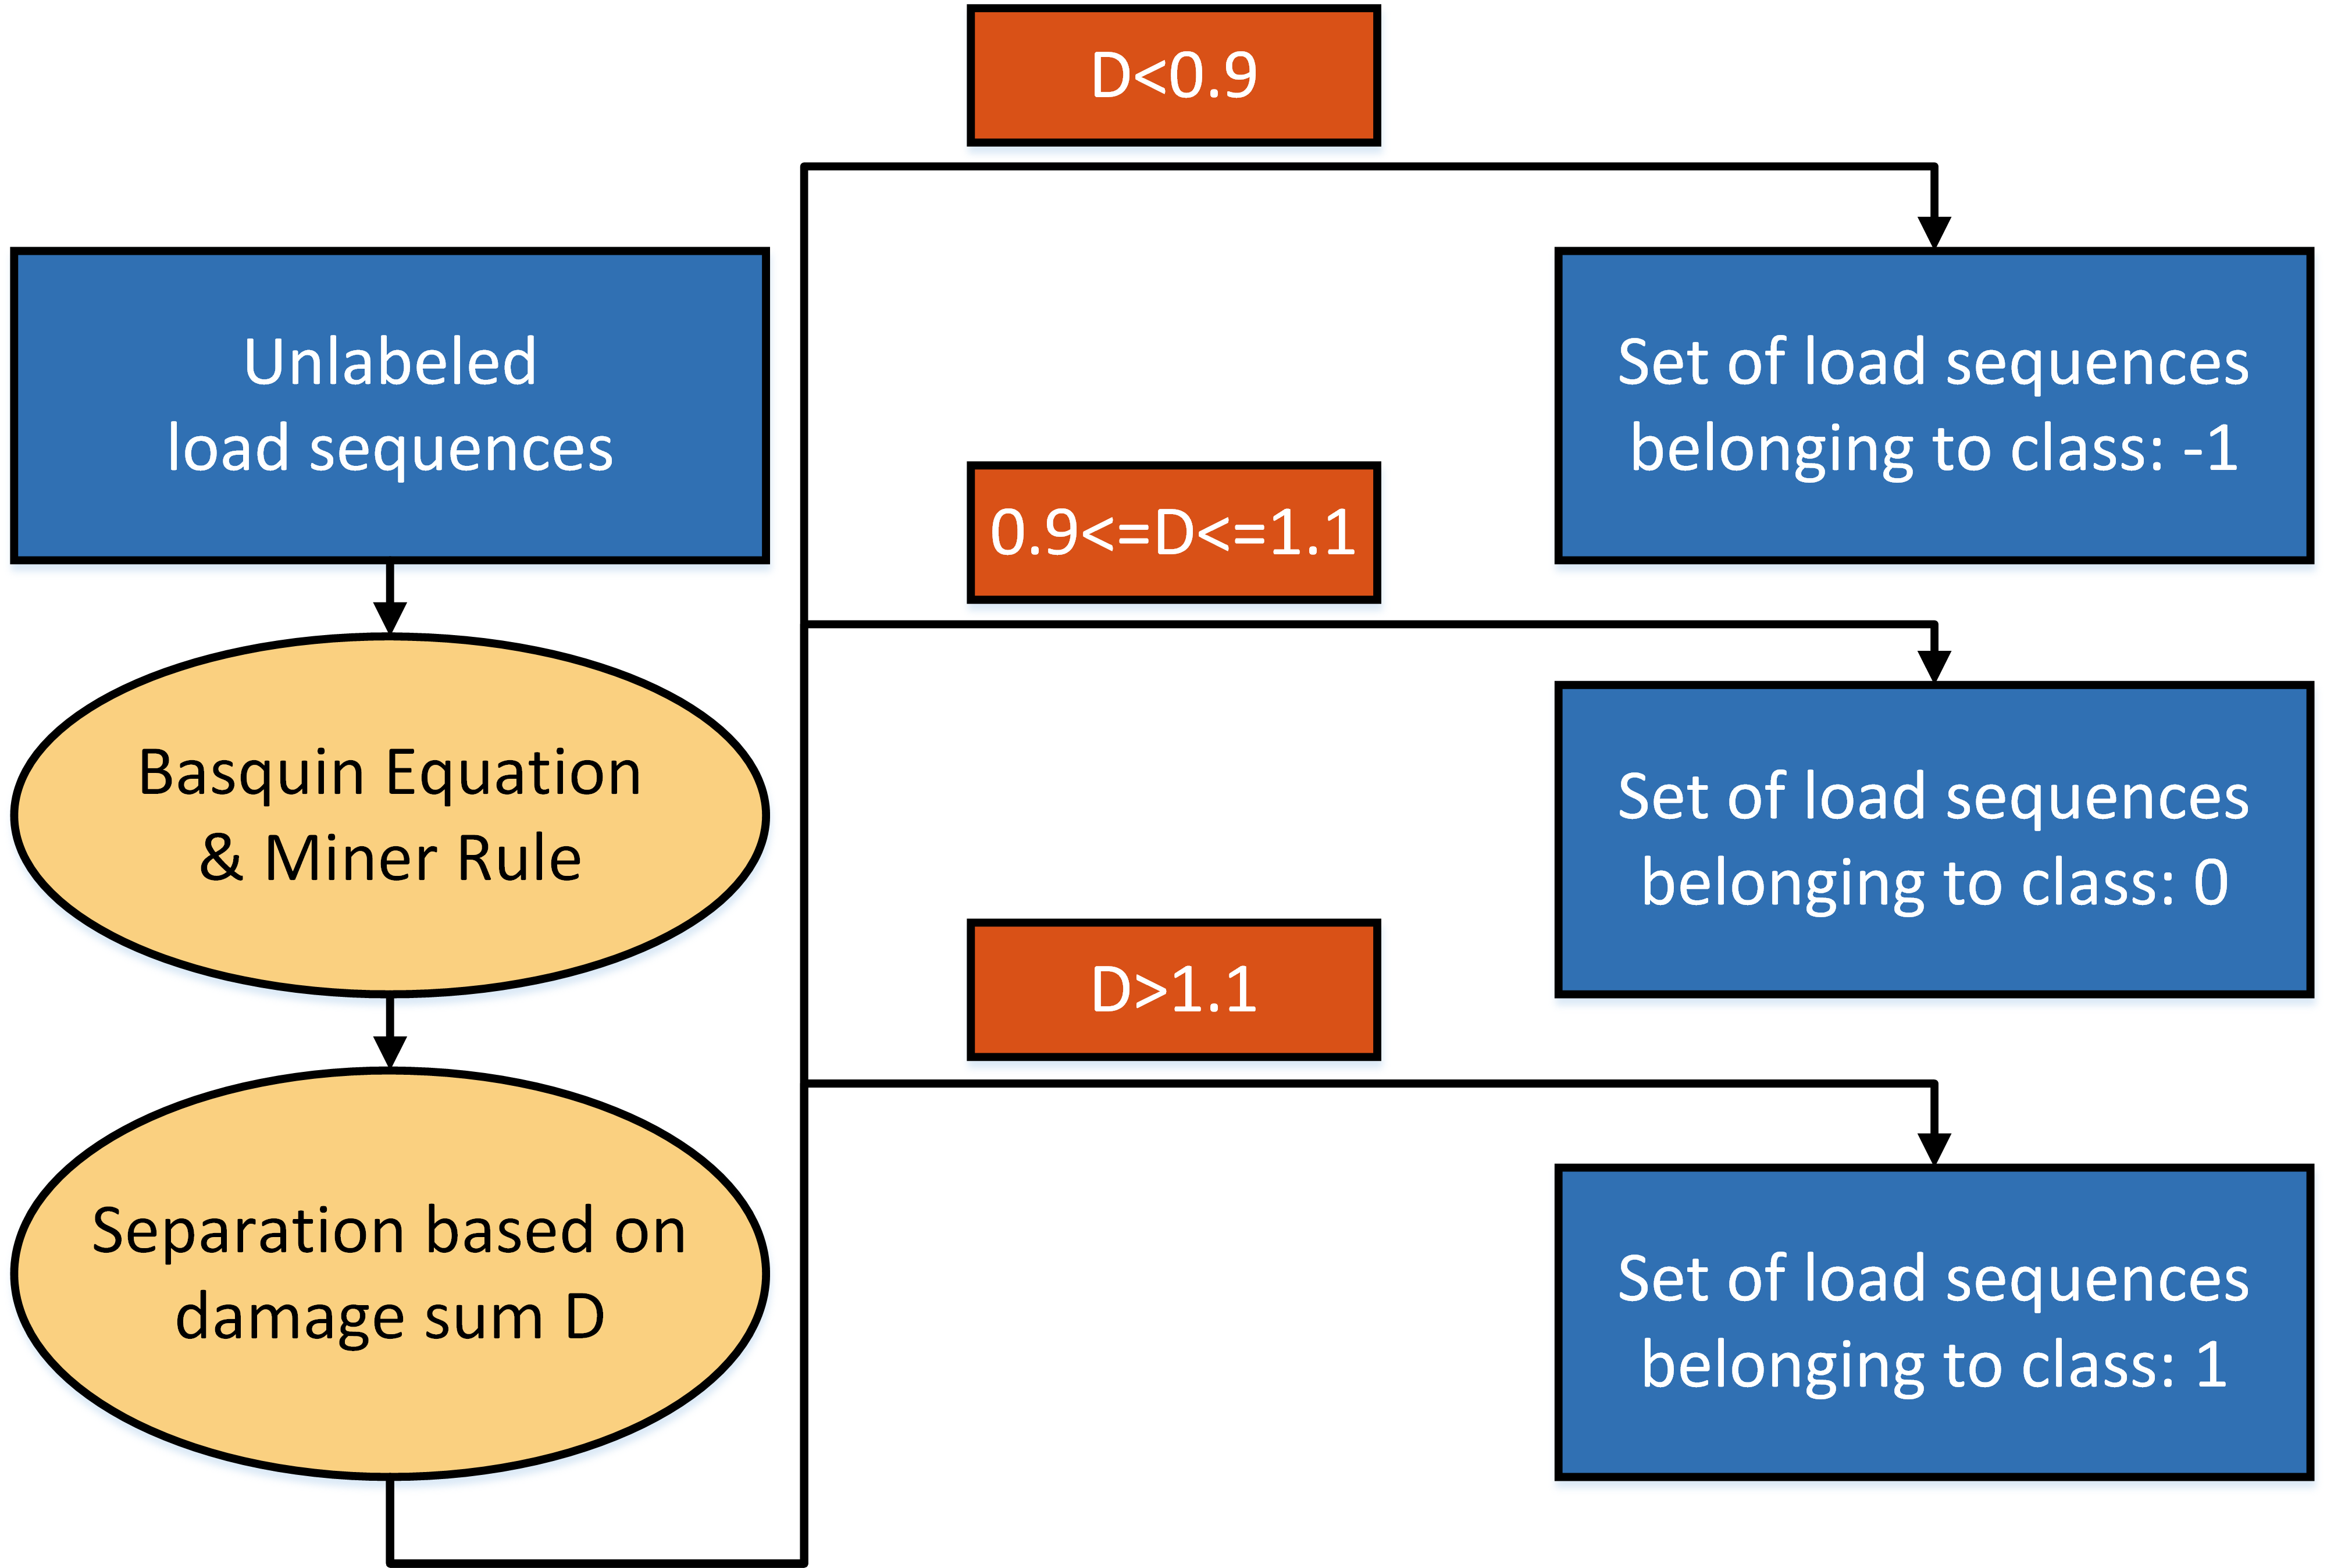
\includegraphics[width=0.8\linewidth]{IMGs/SBC.png}
	\caption{Calculation of damage sum D and separation into classes}
	\label{fig:SBC}
\end{figure}

\begin{table}
	\begin{center}
		\begin{tabular}{|| l | l ||}
			\hline
			\rule{0pt}{2ex}Damage sum D & Class\\
			\hline
			\hline
			\rule{0pt}{2ex}D < 0.9 & Class: -1\\\hline
			0.9 <= D <= 1.1 & Class:  0\\	\hline
			D > 1.1 & Class:  1\\\hline
			\hline
		\end{tabular}
		\caption{Label assignment based damage sum D at failure}
		\label{DamageClass}
	\end{center}
	\vspace{-4mm}
\end{table}


Figure \ref{fig:SBC1} gives a more visual representation of how the different load sequences are separated into classes. Note that short sequences can have a higher damage sum D as it is not dependent on just the number of cycles but also on the load level. The end of a sequence is the point where the gear failed. 

\begin{figure}[H]
	\centering
	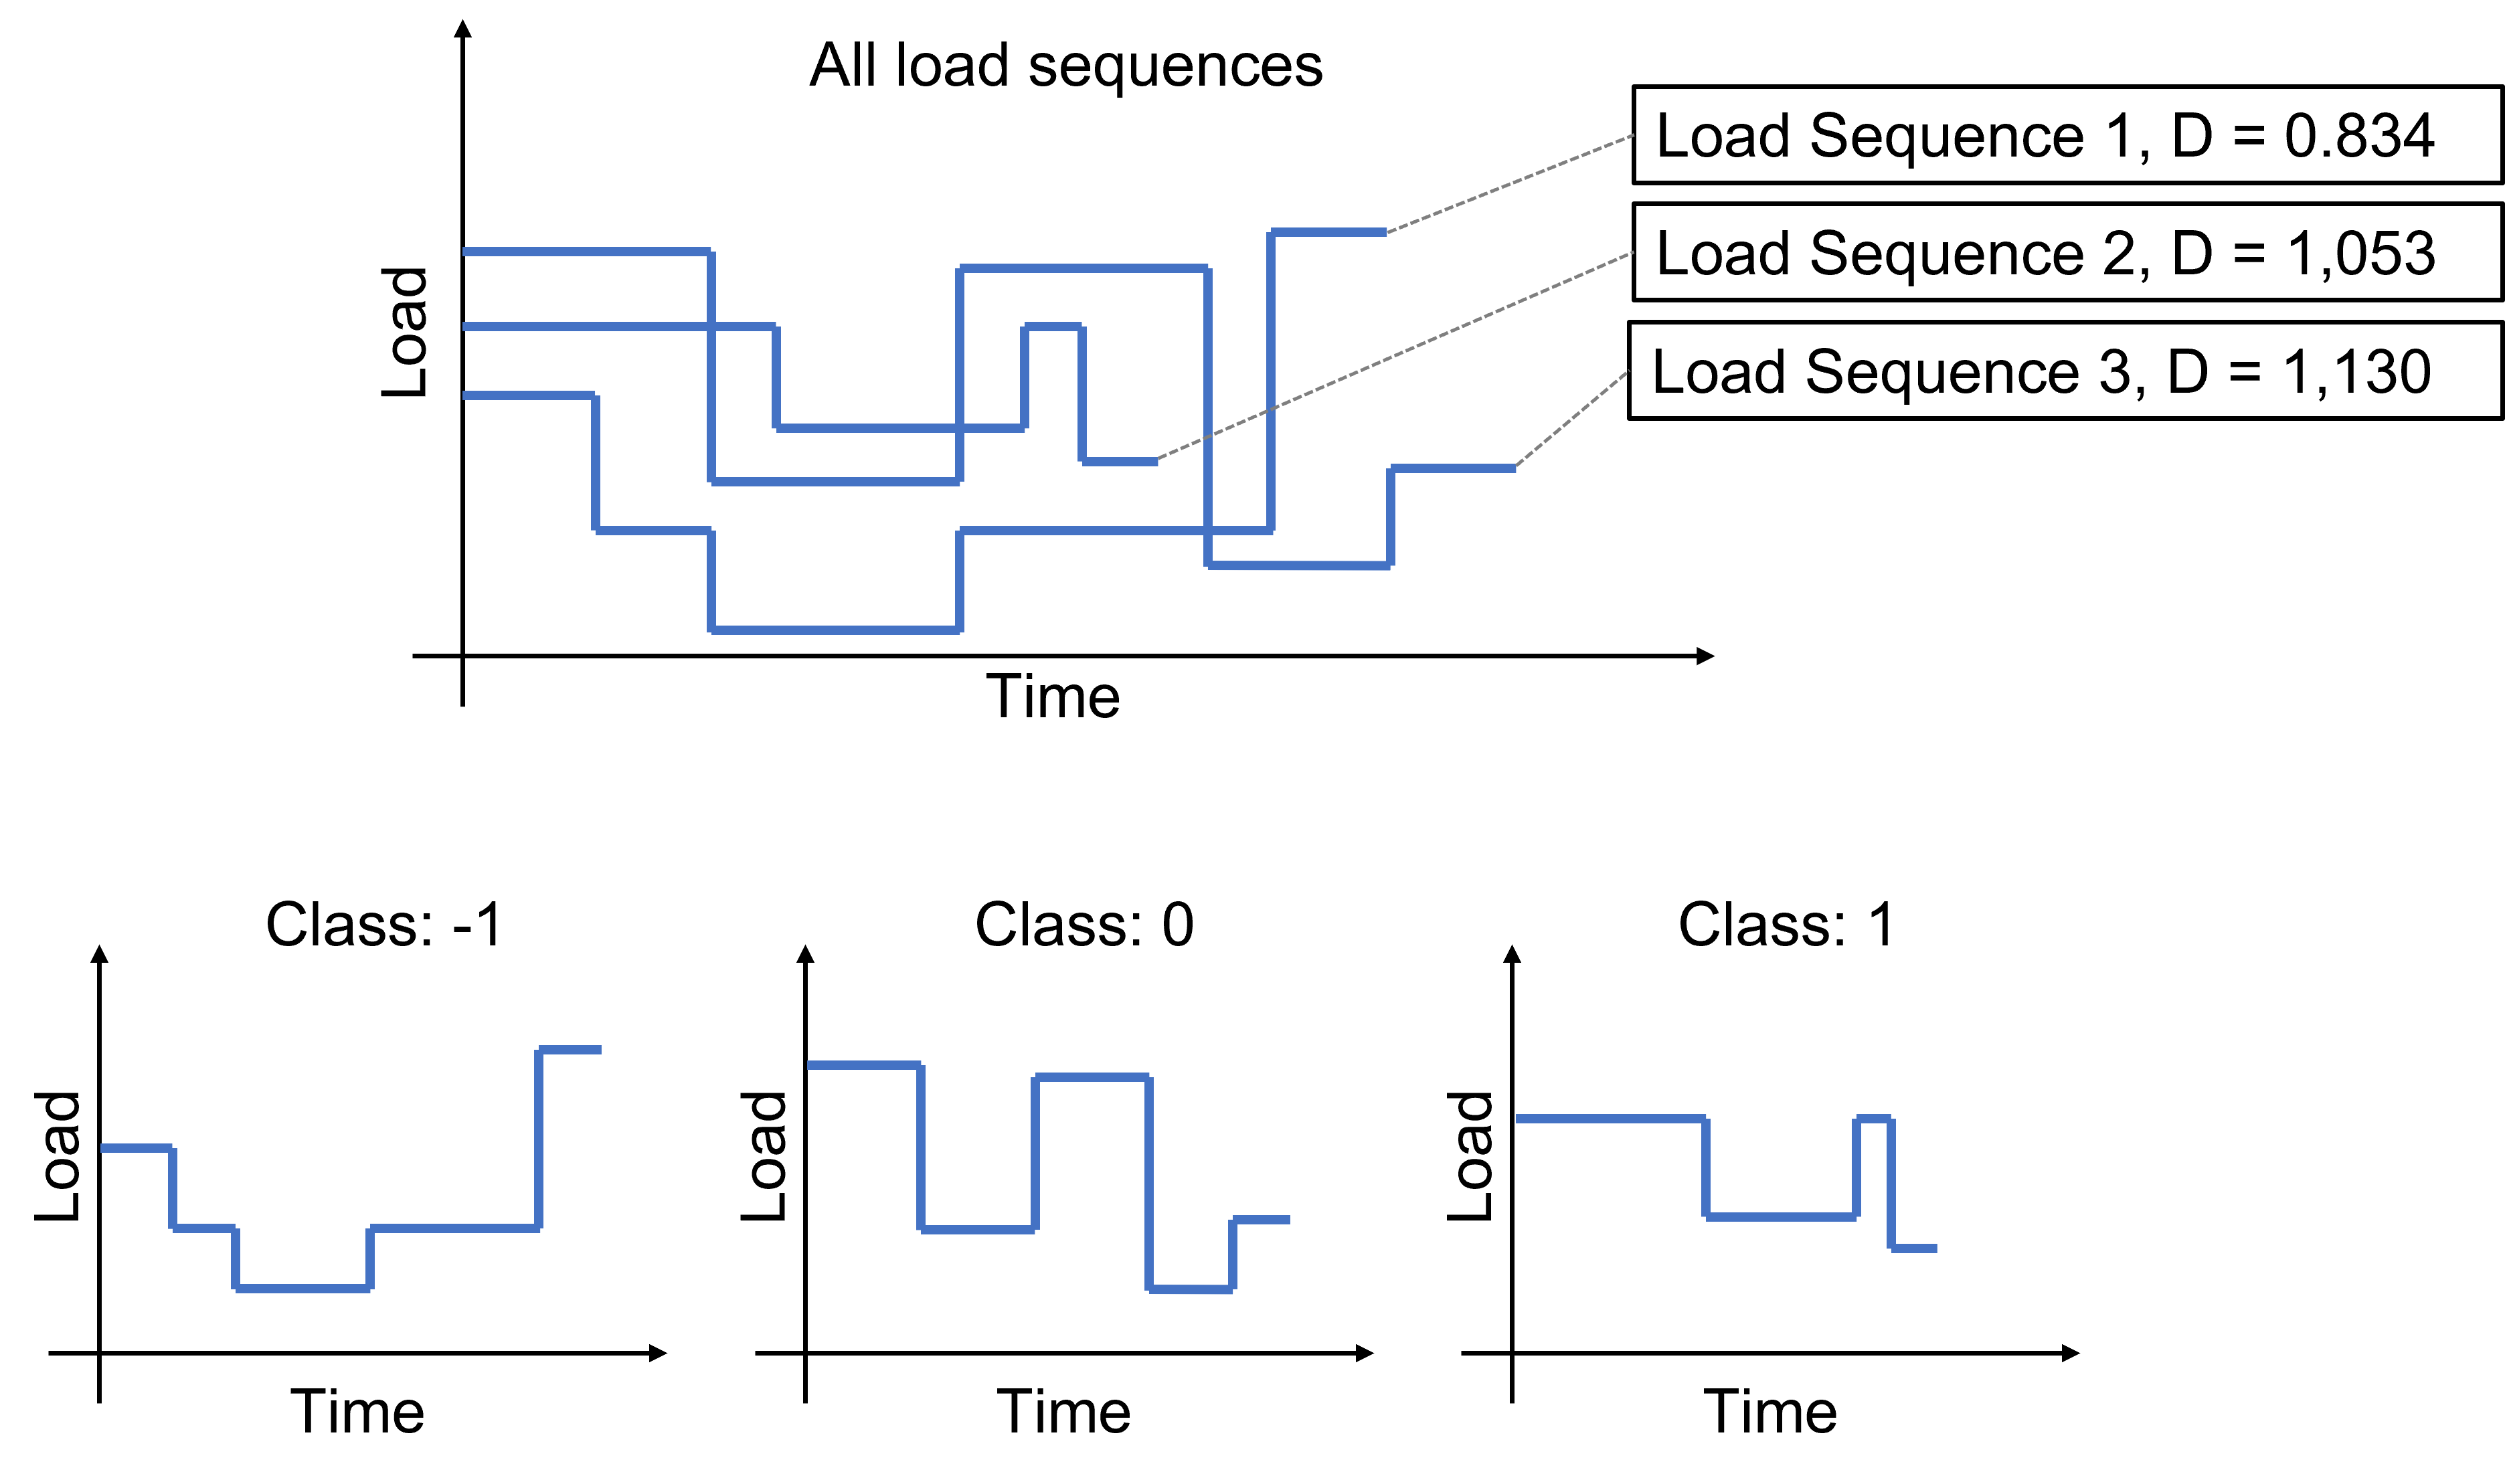
\includegraphics[width=0.9\linewidth]{IMGs/SBC1.png}
	\caption{Separation of load sequences based on classes}
	\label{fig:SBC1}
\end{figure}

\subsection{Pre-processing for Classification}\label{prep_class}
Before the classifier can be trained, further pre-processing steps need to be performed. The first is data augmentation (DA), and the second is dimensionality reduction. 

The goal of DA, as mentioned in chapter \ref{DAUG}, is to increase the diversity and size of a data-set. This gives the classifier more data to train on and reduces the risk of over-fitting.
This step is especially important if the sample size is small. Due to the physical nature of the problem, multiple aspects have to be considered when performing DA.

If the data-set is very limited, DA will only slightly boost the performance, as the inherent problem is the lack of data. Further, if DA is performed, the accumulated damage sum D of the total load sequence must not change significantly. If a load sequence is changed significantly and in such a way alters the damage sum D, the inherit properties of the load sequence can be lost. The classifier relies on characteristics that correlate to the label of a load sequence. Significantly changed characteristics will confuse the classifier in training and lead to poor performance.


The same principle applies to the step of dimensionality reduction. ML models perform better with input vectors that are short and have values in a similar range. One possible option for dimensionality reduction is selecting every \(n^{th}\) point in a sequence.
When analyzing, if the reduced sequence has the same damage sum D as the original, the numerator of the Miner rule must be multiplied by the step-size that was used to select every \(n^{th}\) point. For example, if every 200\(^{th}\) point is selected, the step-size is 200. When calculating the damage sum D on the reduced sequence with equation \ref{acc} the numerator must be multiplied by 200.


Figure \ref{fig:DAUG} shows the steps of DA and dimensionality reduction, including a feedback loop to ensure that the augmentation and dimension reduction do not change the damage sum D.
It is important that the comparison is performed after each individual step. In a worst-case scenario, the augmentation and dimensionality reduction change the damage sum in opposite directions. In this case, the final damage sum is equal to the original load sequence, but the characteristics are all lost.

 
\begin{figure}[H]
	\centering
	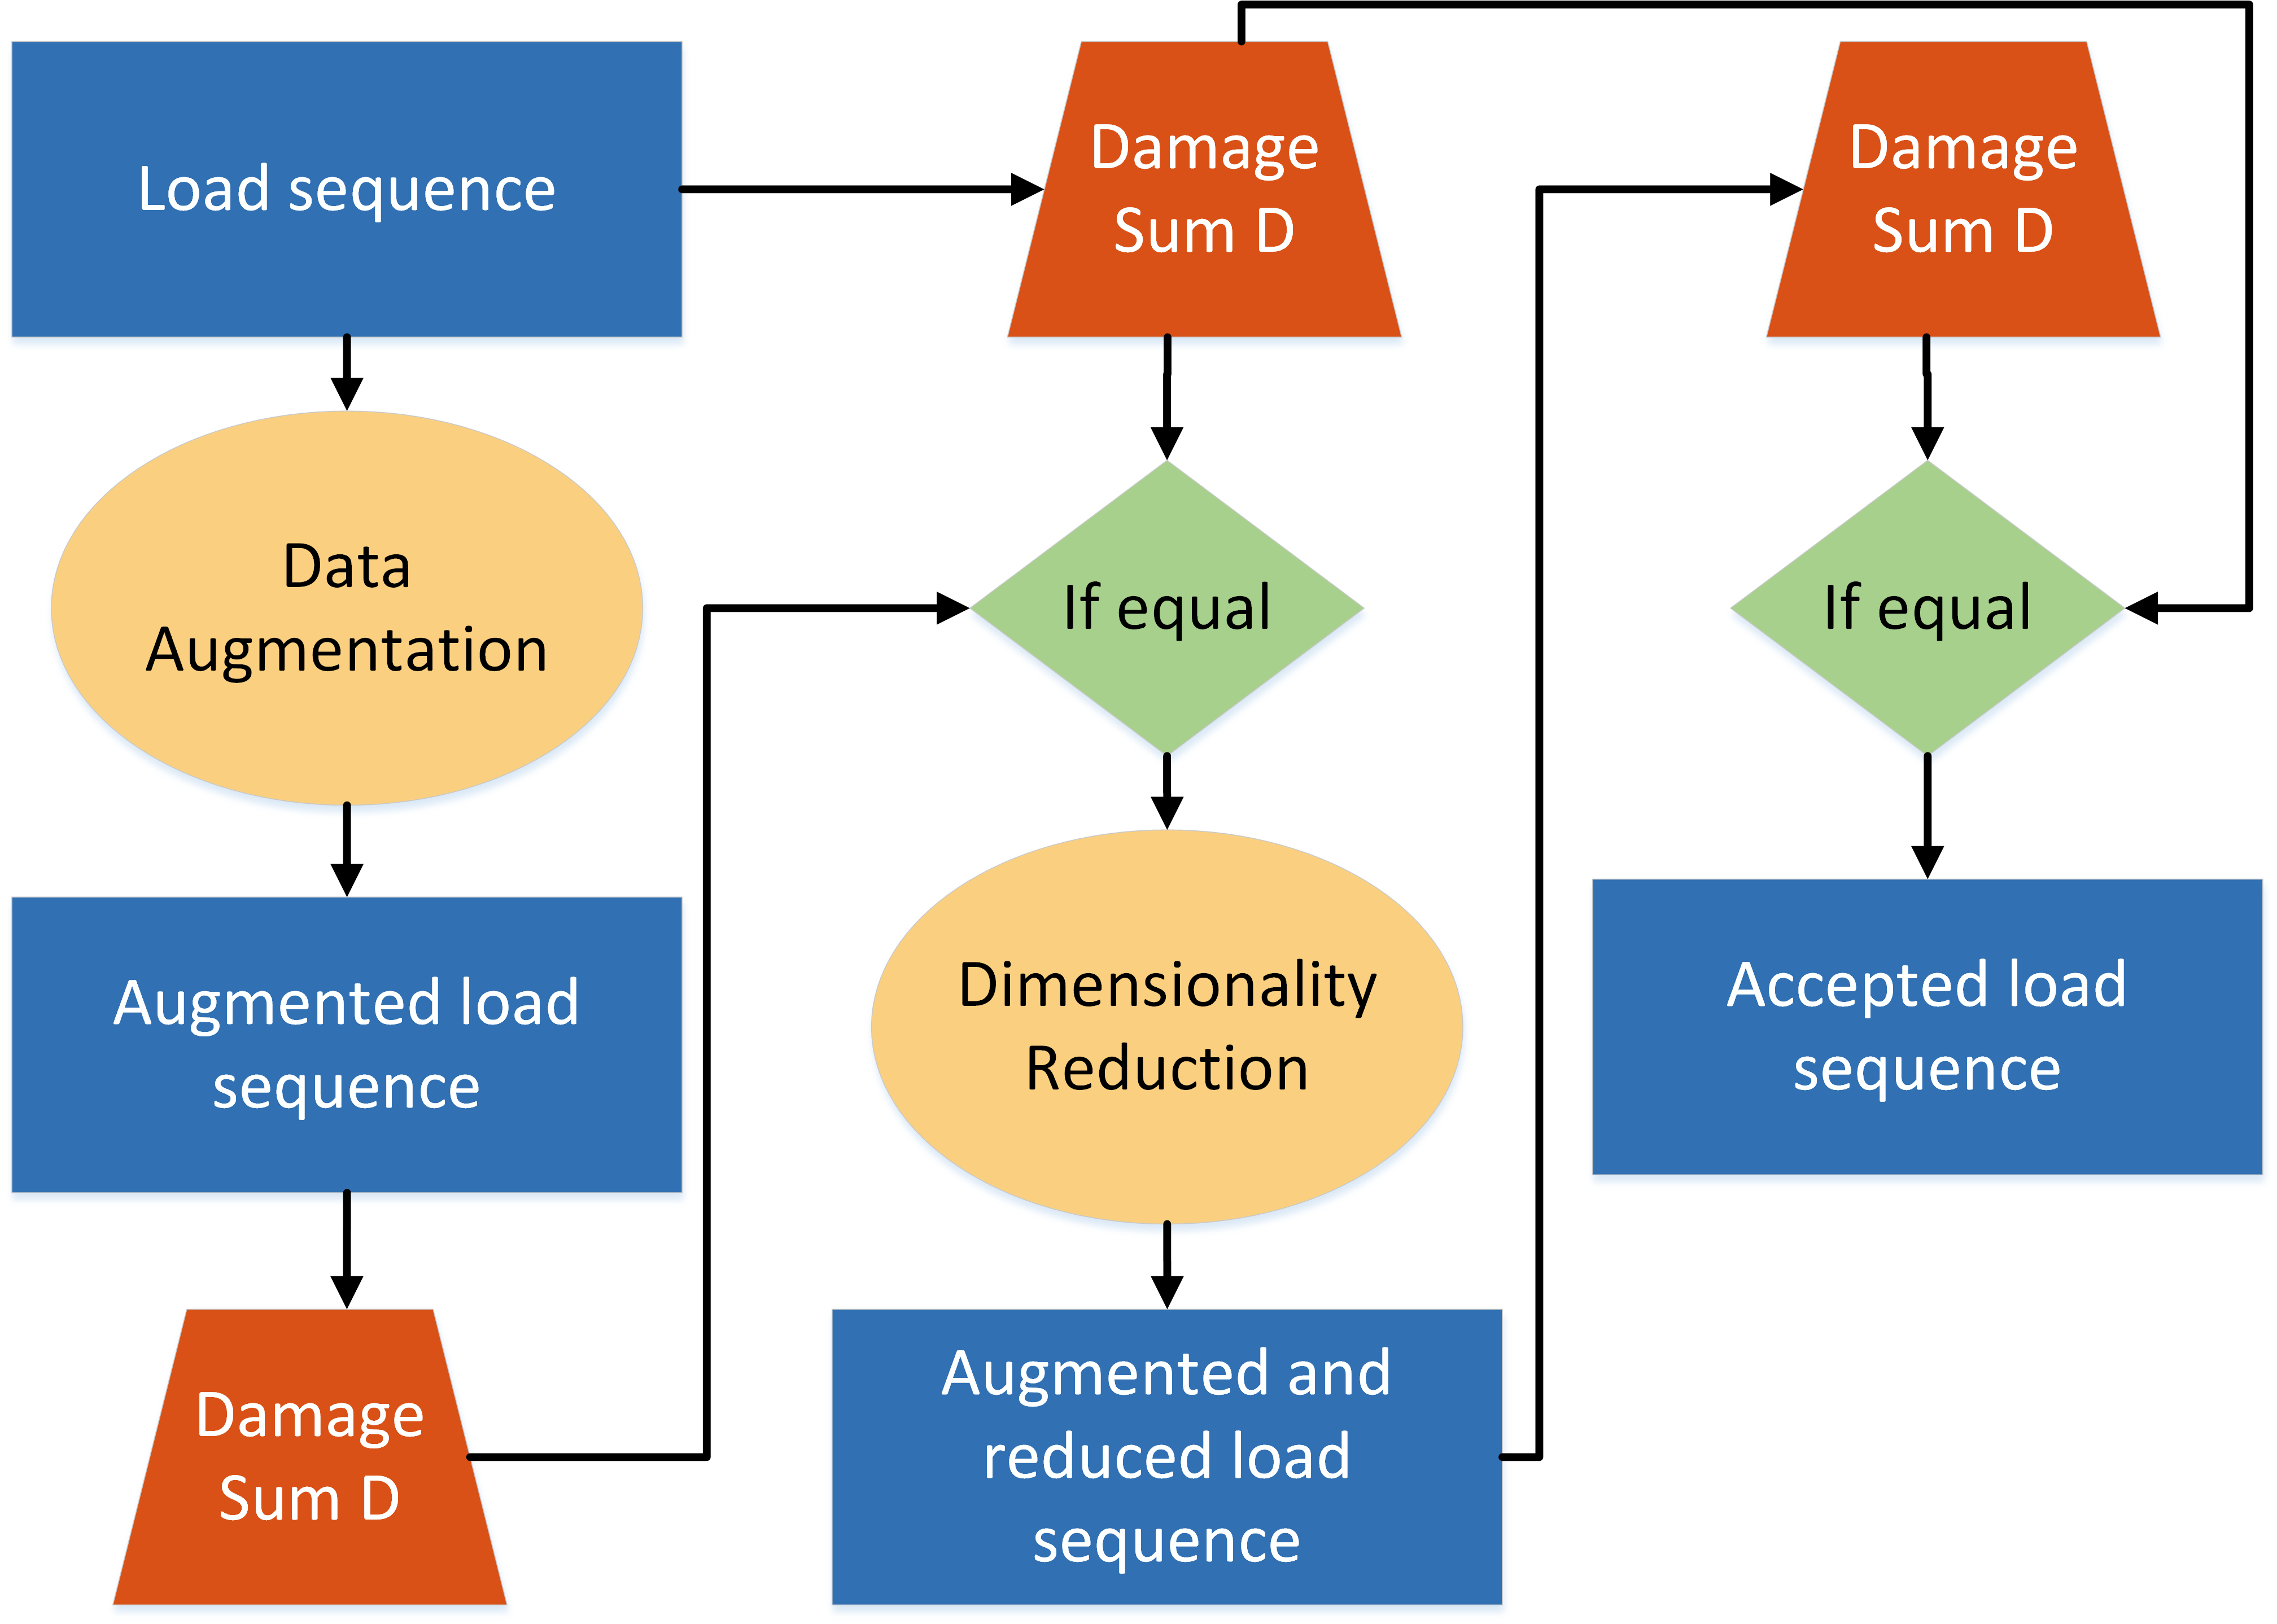
\includegraphics[width=0.8\linewidth]{IMGs/DAUG.png}
	\caption{Data Augmentation and Dimensionality Reduction with feedback loops}
	\label{fig:DAUG}
\end{figure}

Note that the equality of th damage sum D after DA is the optimal case. Finding DA techniques that vary the load sequences but keep the damage sum D the same is very difficult. To work around this problem, a load sequence is regarded as acceptable if the damage sum D differs by 10 \% in any direction.


Figure \ref{fig:UL} shows the issue of just selecting every \(n^{th}\) point for dimensionality reduction. By missing significant portions of the load sequence, peaks and low spots can be missed or accentuated. Multiplying the number of cycles in the Miner rule with \(n\), is the same as expanding every cycle by \(n\) and using the Miner rule without multiplication. The two graphs in \ref{fig:UL} show that the expanded load sequence has significant differences and that all characteristics have been lost. By comparing the damage sum at each step to the original, such cases can be found and not taken into the training data-set. Another way of reducing this problem is to select a smaller step-size which in turn will increase the feature vector size that will be used as an input. 

\begin{figure}[H]
	\centering
	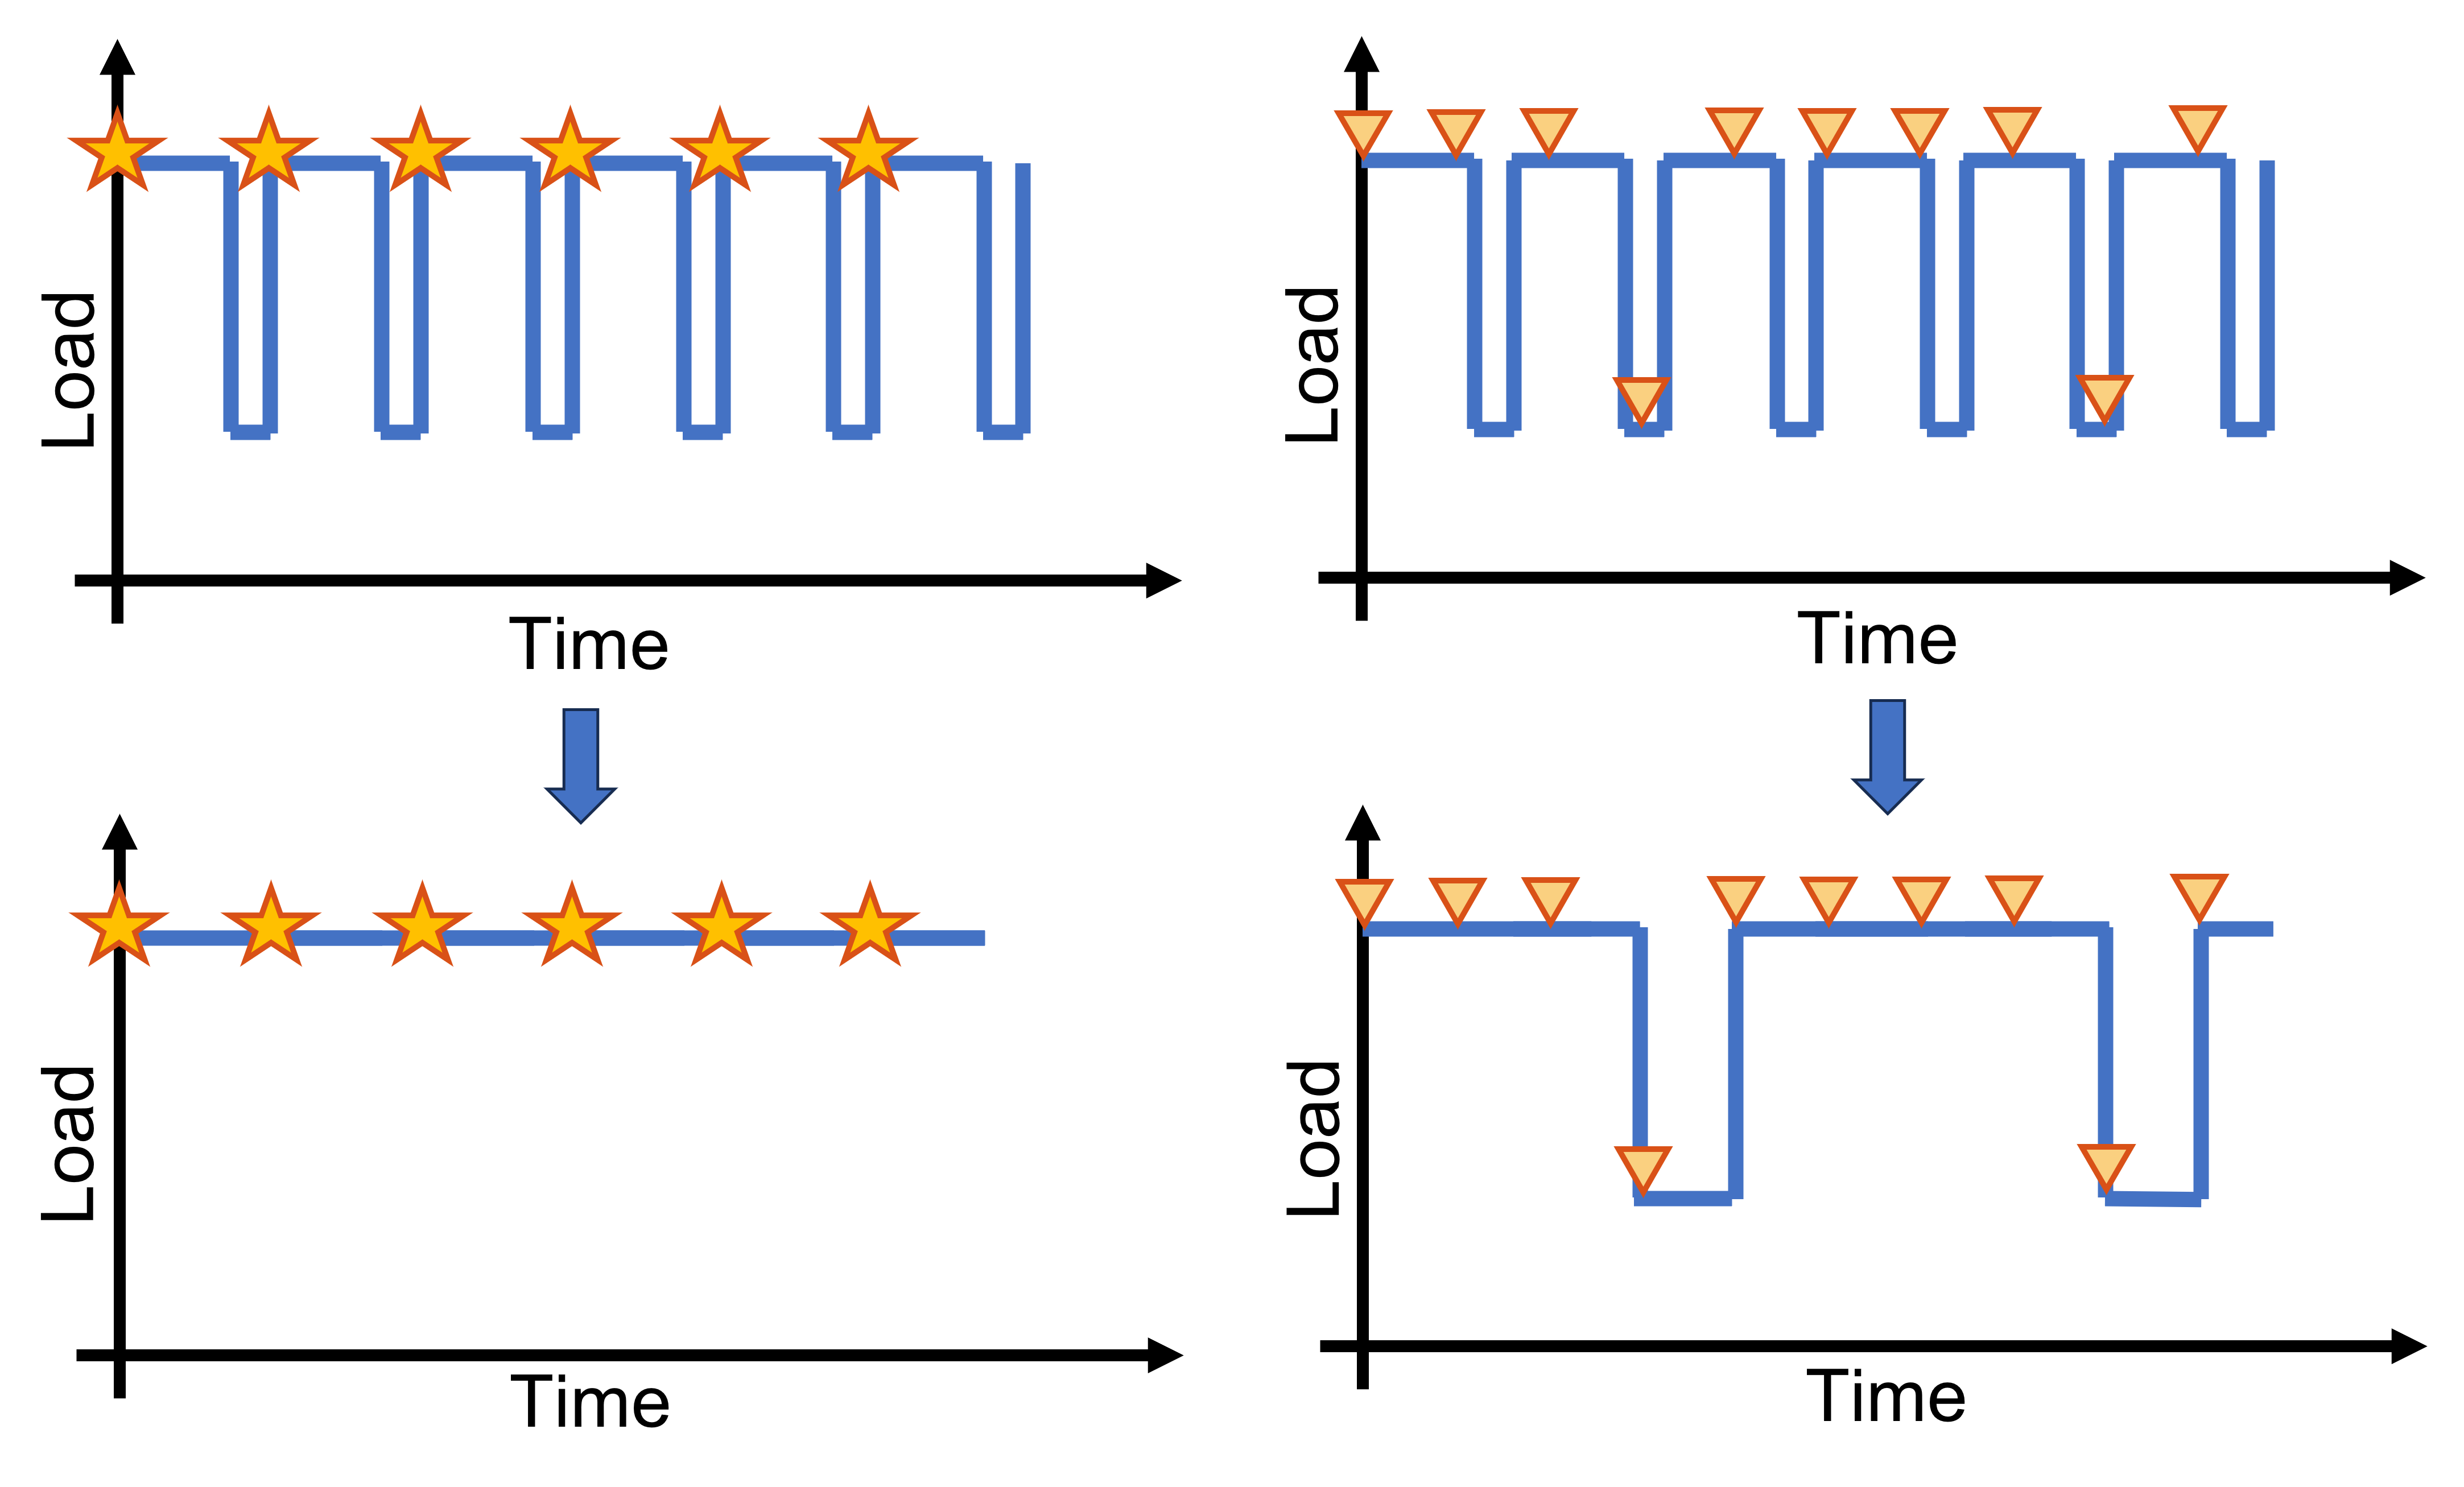
\includegraphics[width=0.8\linewidth]{IMGs/Unlucky.png}
	\caption{Danger of Dimensionality Reduction by selecting equidistant points}
	\label{fig:UL}
\end{figure}
 
\subsection{Usage of the Classifier}
The classifier is used as a method to classify an unfinished load sequence, whether it is part of the more damaging, less damaging ones or correctly assessed ones. After the performed steps of separation into classes, DA and dimensionality reduction, the load sequences require a last pre-processing step. At the moment, the load sequences are in their full length and have a different damage sum D.
If an unfinished sequence, of a gear that has not yet suffered fatigue damage needs to be classified, the comparison has to be made with sequences that have the same damage sum~D as the unclassified sequence. In other words, if a current sequence is at damage sum D = 0.6 and it is of interest if this is a correct estimate, it needs to be compared to other load sequences at D = 0.6.
 
To do so, all sequences are cut (shortened) so that they all end at the same damage sum D. 
With those sequences and their labels, the classifier is trained.
After training, the classifier can take the unfinished sequence that underwent the same dimensionality reduction as the rest and predict a class-label. 
Based on the predicted class label, a conclusion can be drawn if the calculated damage sum D based on the Miner rule is more on the conservative or lenient side. Figure \ref{fig:Class} shows the steps of the last pre-processing steps and the classification of a sequence.


\begin{figure}[H]
	\centering
	\includegraphics[width=0.9\linewidth]{IMGs/Class.png}
	\caption{Load sequence adaption, training and final classification }
	\label{fig:Class}
\end{figure}


Figure \ref{fig:Shortened} gives a visual representation of how load sequences of class 1 (D>1.1) are adapted when the unfinished sequence has the damage sum D of 0.6 according to the Miner rule.
All recorded points after D=0.6 are deleted in every load sequence. By doing so, the sequences are shortened. These sequences are then used as training data to predict the label of the unlabeled sequence. The same is done to the sequences of classes 0 and 1.

Note that if an unlabeled sequence is past a certain damage sum D, the classification will become more uncertain. For example, if a sequence has a damage sum D = 0.85 but most of the sequences in class -1 end at 0.8, there are significantly fewer data samples that can be used for training in that class. 

For a classification of a load sequence that has a very low damage sum D (for example 0.3) the classification also becomes very uncertain, as it is possible that not enough characteristics are present in a load sequence that could place it in one category with high certainty.
So there exists a sweet spot that is determined by the number of training-elements in each class and the damage sum D of the unknown label.

\begin{figure}[H]
	\centering
	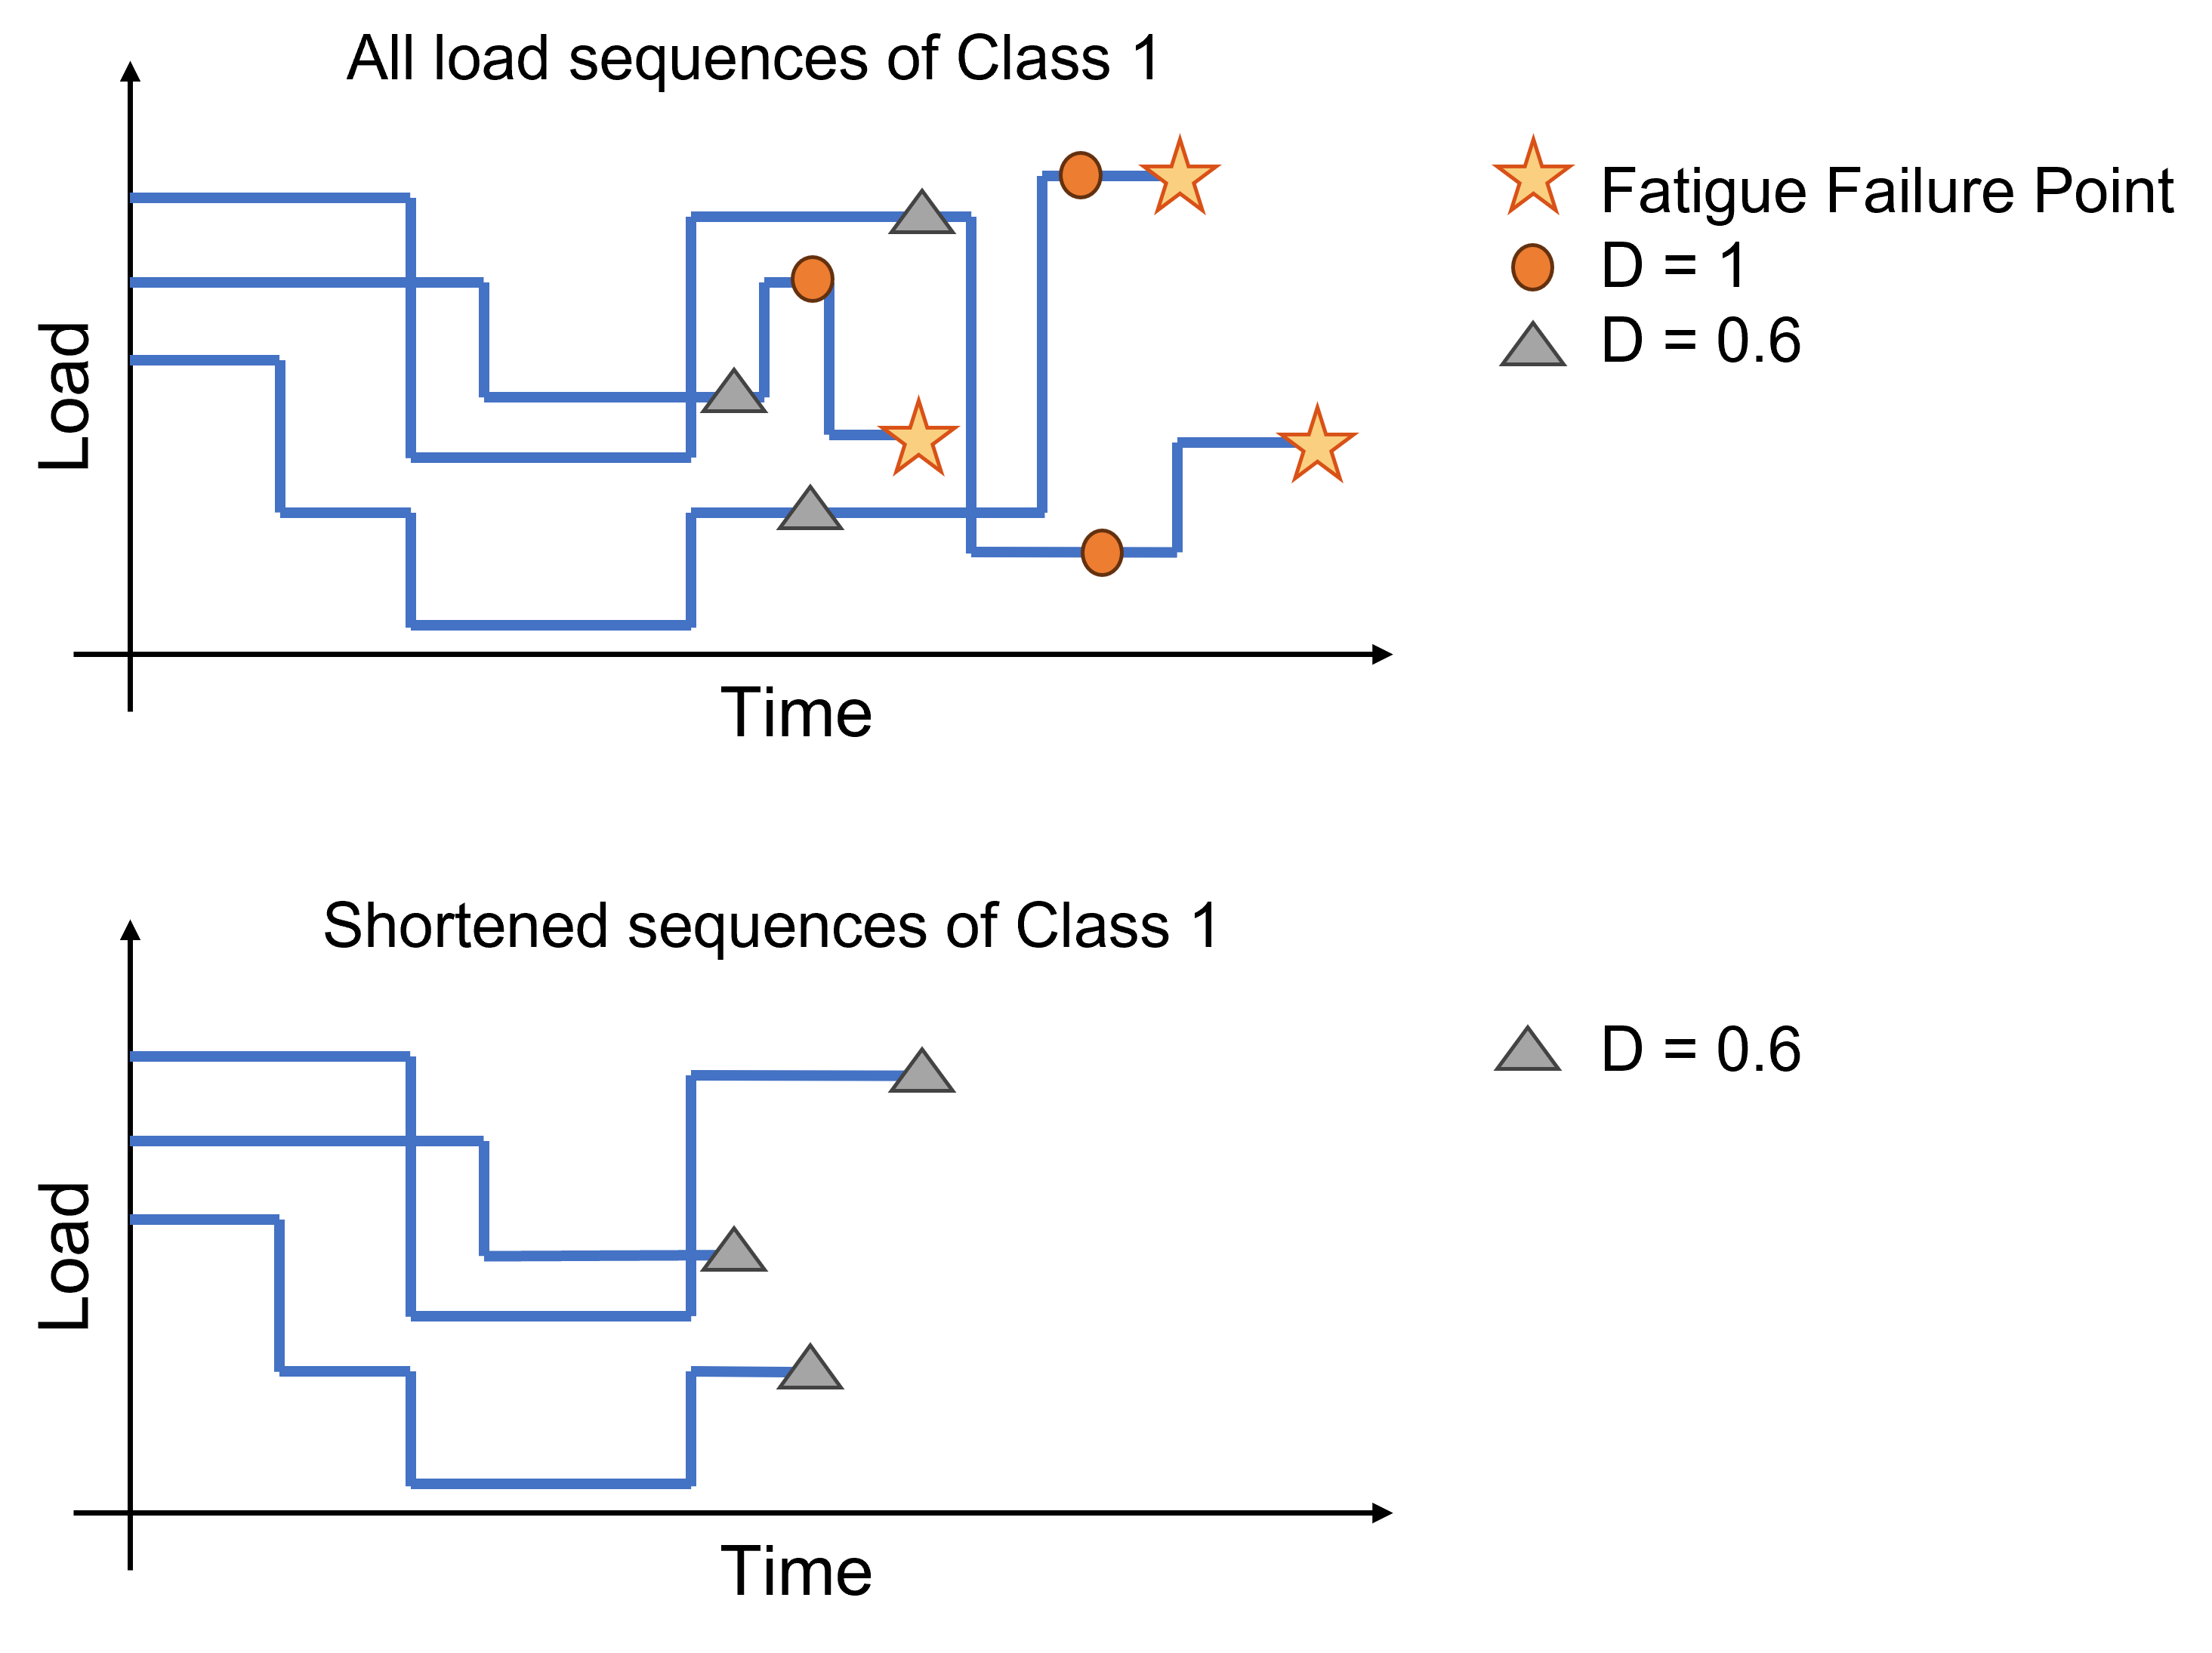
\includegraphics[width=0.8\linewidth]{IMGs/Shortened.png}
	\caption{Load sequence shortening}
	\label{fig:Shortened}
\end{figure}

\subsection{Problems in Classification of Sequences}
One of the problems in classifying sequences is the difference in length of those sequences. The original recordings can have a different number of cycles, which makes it difficult to use them as input-vectors. Most algorithms require a constant input-vector size for training and validation. This problem can be circumvented by pre-filling each augmented and reduced sequence with zeros to a uniform length, or using an approach that can work with sequences of different sizes. 


The only problem remaining is the prediction of an unseen sequence that might be longer than any other sequence seen in training.
This problem can be solved by pre-pending more zeros to create a buffer for the ability to classify longer sequences than those present in the training data.



\section{Regressor for SOH-Prediction}
The regressor is used as a linear extrapolation model that calculates the SOH of a gear. The SOH can be interpreted as a value for how soon the gear is expected to fail. For example, if the Miner rule calculates a damage sum D equal to 0.8, the classifier assigns a class label of 1 (not damaging load history), and the regressor calculates a SOH of 0.9, the gear is expected to be able to withstand higher loads but not for a very long time. In that case, it is expected that the damage sum D will accumulate past unity, but will be limited in the number of cycles it can withstand. 

\subsection{Data-set for Regressor}\label{PrRe}
If an unfinished load sequence is classified into a class, for example, class 1, the regressor will only be trained on the load sequences belonging to that class. Each augmented load sequence is iteratively selected, and n different, randomly determined points are chosen. These points are transferred to the label function of that sequence to determine the label (SOH) of that sequence snipped from the beginning up to that point. The selected snippets are then saved and used as training data for the regressor. 
Figure \ref{fig:dataregressor} shows the process of creating data samples from one load sequence.

\begin{figure}[H]
	\centering
	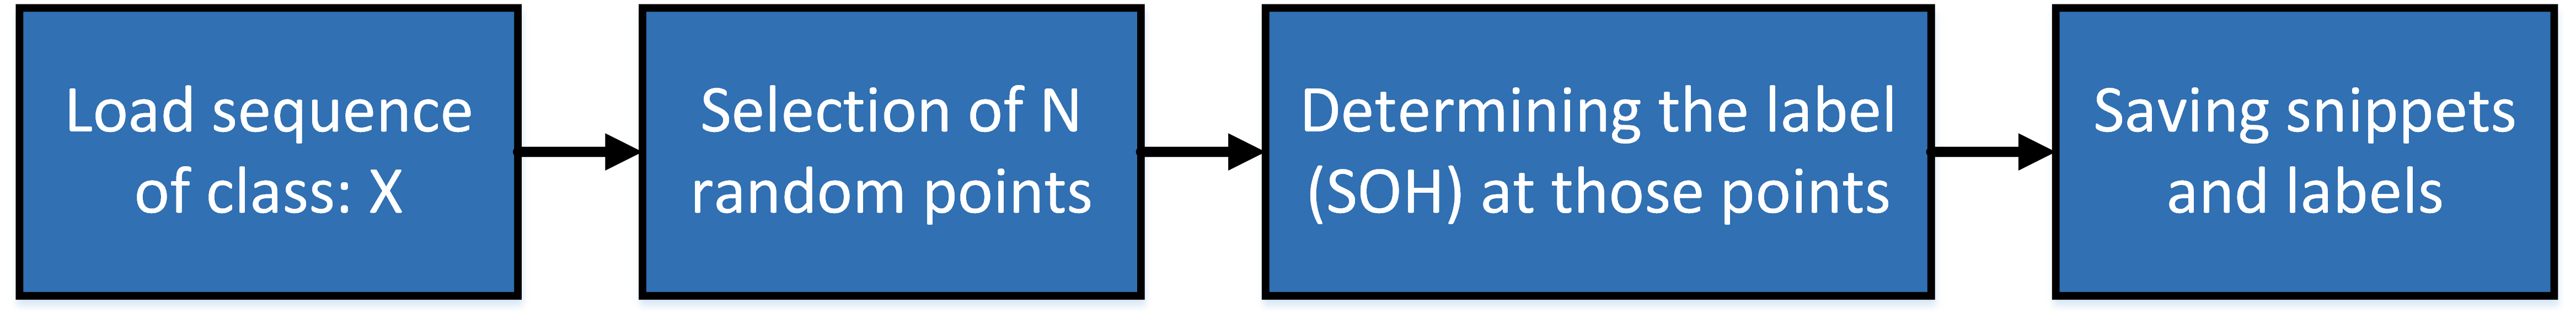
\includegraphics[width=0.85\linewidth]{IMGs/dataregressor.png}
	\caption{Data-set generation process for the regression data-set}
	\label{fig:dataregressor}
\end{figure}

Figure \ref{fig:4elems} gives a visual example of how three elements and the appropriate labels are created from one load sequence. The number of created elements can be freely defined.

\begin{figure}[H]
	\centering
	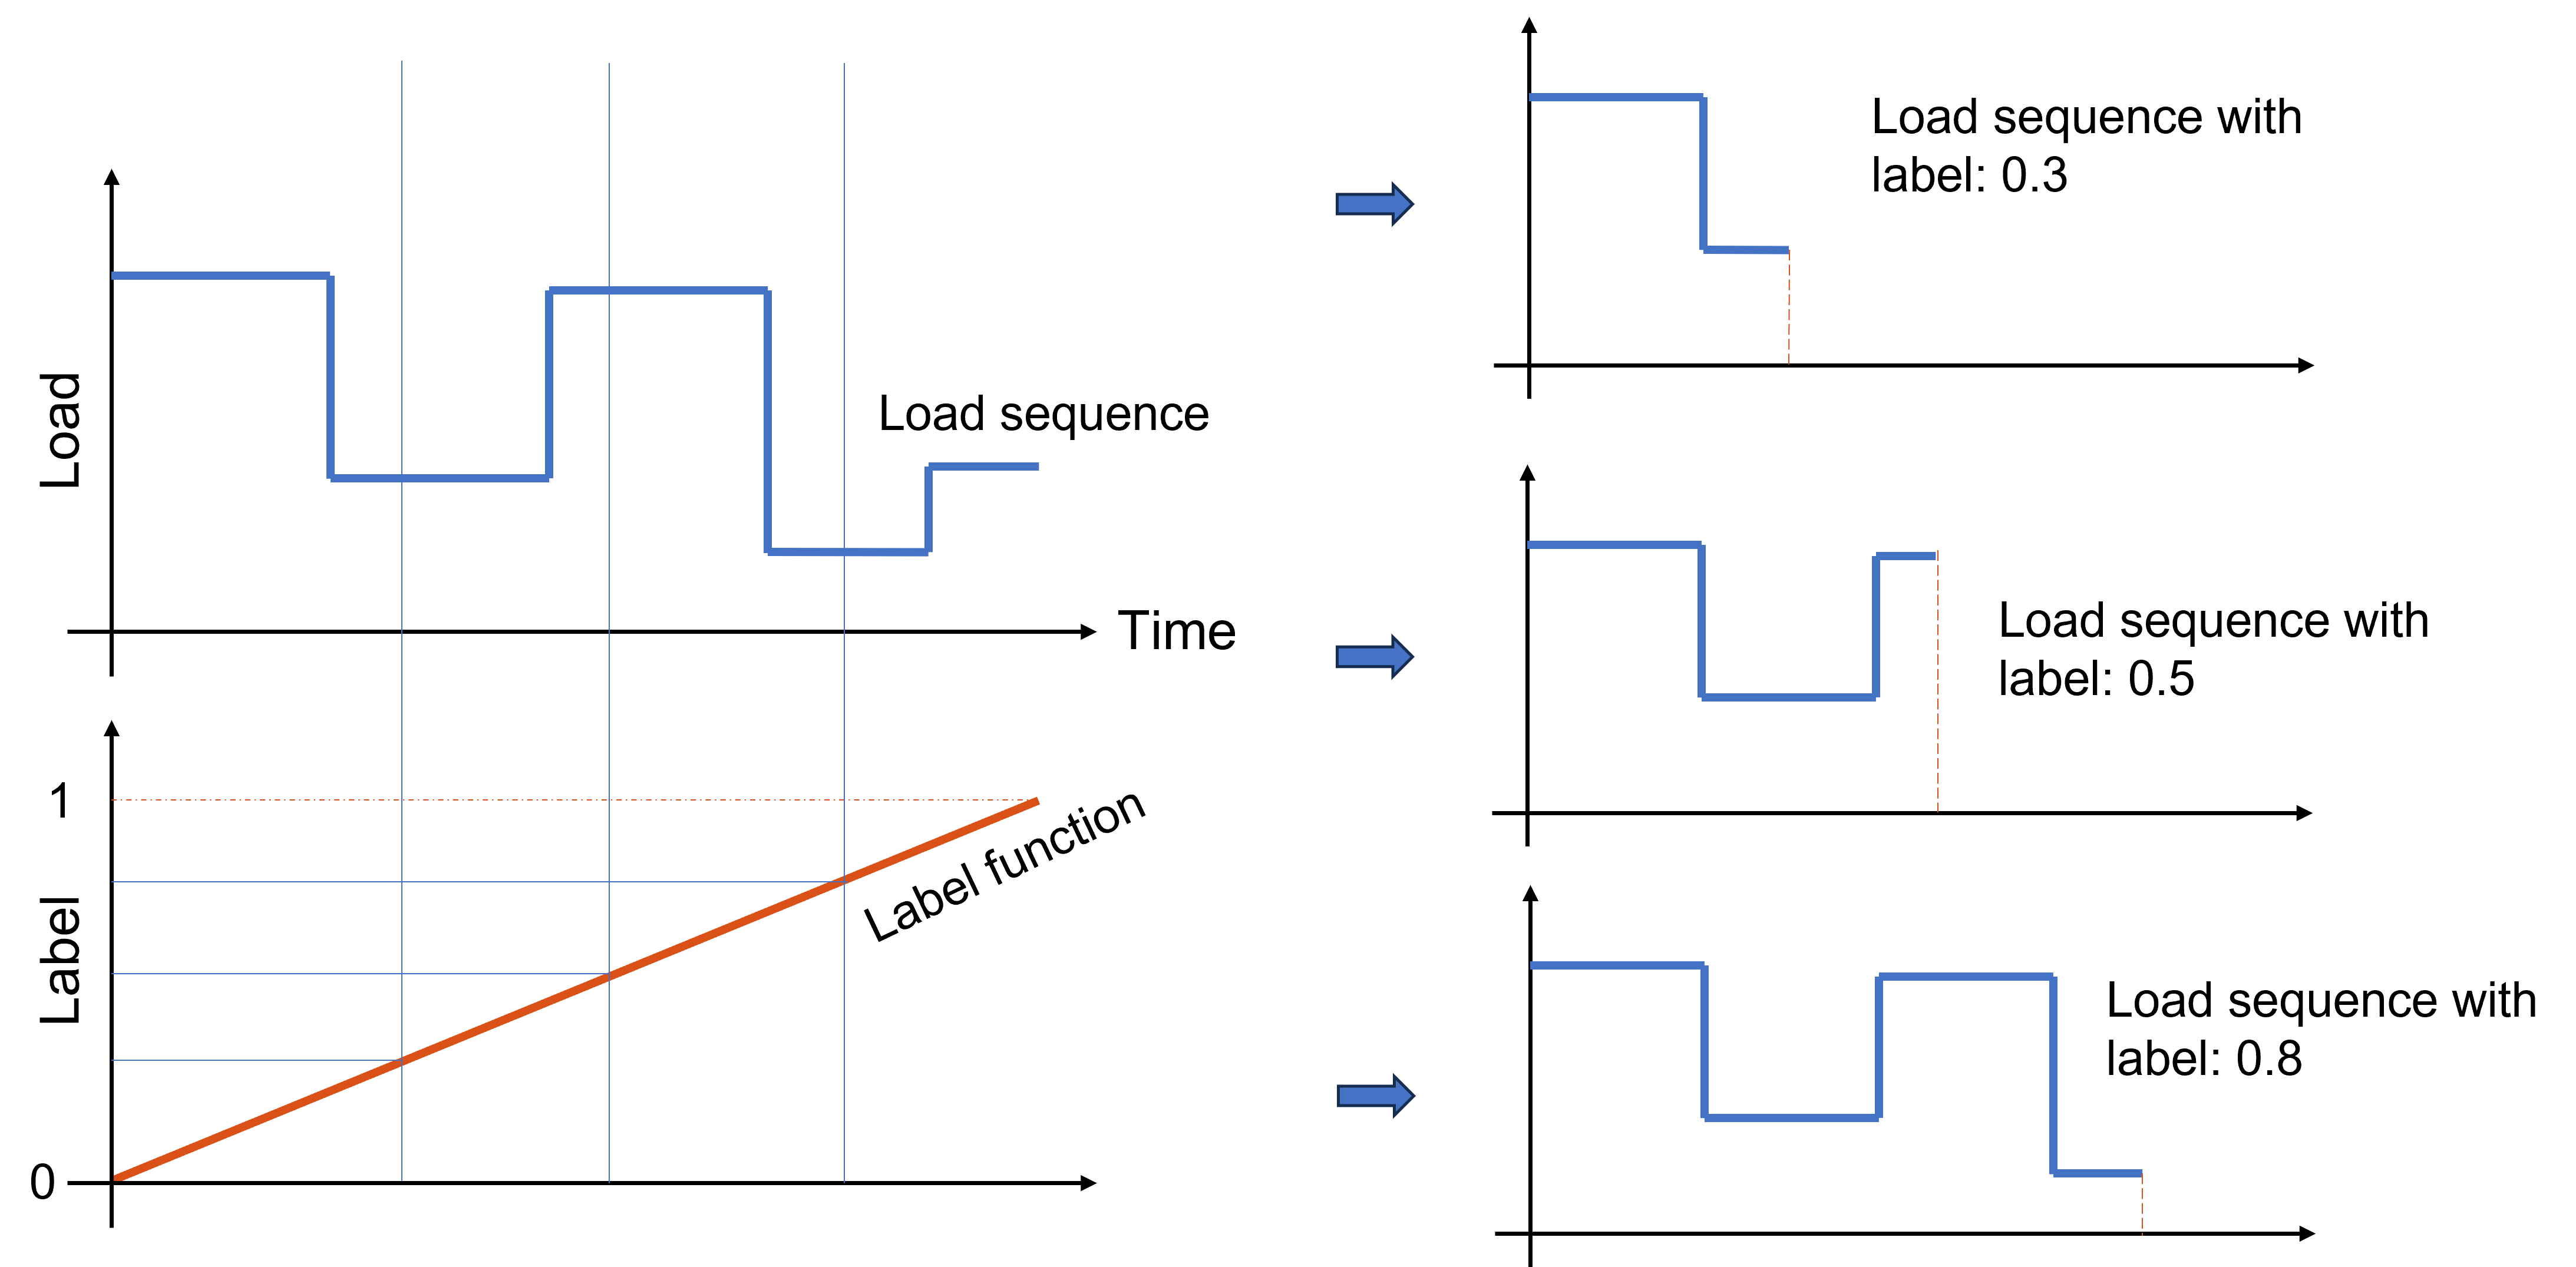
\includegraphics[width=0.95\linewidth]{IMGs/4elems.png}
	\caption{Creation of three elements with the help of the label function}
	\label{fig:4elems}
\end{figure}
\subsection{Training the Regressor}
The created training data-set has the same structure as the classification trainig-set. The sections are now of different lengths, not only because of the different number of cycles but also because of the different selected points. The regressor must either be able to accept input vectors of different sizes or each sequence needs to be pre-filled with zeros (zero-padding) to bring all elements to the same length.
\section{Summary of the Proposed Method}
The goal of the proposed method is to get a confidence value regarding the calculated damage sum D according to the Miner rule. It achieves that by first classifying a sequence into a category that represents the influence of the order of the loads. By doing so, it can be determined if the Miner rule is giving a conservative or lenient estimate. The classification is based on a supervised learning algorithm that uses load sequences that failed before and after reaching an accumulated damage sum D equal to unity. The second step is a regressor that predicts a state-of-health, which is a value calculated by extrapolating the expected failure point in time based on the load sequences that have the same effect based on the order of loads. With these two values, the confidence in the calculated damage sum D can be evaluated.
Table \ref{cases} gives an overview on how to interpret the different combinations of the two values. 

\begin{table}
	\begin{center}
		\begin{tabular}{|| r | l | l ||}
			\hline
			\rule{0pt}{2ex}Class & SOH & Effect\\
			\hline
			\hline
			\rule{0pt}{2ex}-1 (Very damaging)&  0,5 & will fail at D<1, but can withstand many cycles with low load\\\hline
			1 (less damaging)& 0,5 & will fail at D>1, and can withstand many cycles with high load\\\hline
			-1 (Very damaging)&  0.9 & Will fail very soon\\\hline
			1 (less damaging)& 0.9 & Will fail very soon but exceed D=1 if future load are high\\\hline
			\hline
		\end{tabular}
		\caption{Effect of the predicted class and SOH}
		\label{cases}
	\end{center}
	\vspace{-4mm}
\end{table}


\afterpage{\null\newpage}